\documentclass[12pt]{article}

% ---------- Packages ----------
\usepackage[margin=1in]{geometry}
\usepackage{amsmath, amssymb}
\usepackage{graphicx}
\usepackage{booktabs}
\usepackage{caption}
\usepackage{subcaption}
\usepackage{setspace}
\usepackage{authblk}
\usepackage[round]{natbib}
\usepackage{hyperref}
\usepackage{float}

\onehalfspacing

\title{Smoke and Strife: Fire Exposure and Social Conflict in Indonesia}
\author{Hariaksha Gunda}
\affil{The University of Alabama}
\date{Working paper, \today}

\begin{document}

\maketitle

\begin{abstract}
Seasonal land and forest fires blanket much of Indonesia in severe air pollution (``haze'') each year. I ask whether exposure to this fire-driven pollution affects social conflict, using fire activity upwind of each district, where the prevailing wind would carry smoke toward it, as a source of variation driven by wind rather than by local conditions. In districts where conflict is common, more upwind fire reduces monthly conflict events. The effect grows with a district's conflict history measured before the sample period, does not appear for next month's fire, and is robust to excluding the district's own fires and to controlling for local weather. The pattern of declines points to two channels. Protests fall with smoke from fires in other provinces, which cannot draw on local security forces, consistent with a direct effect of smoke. Events carried out by security forces fall about five times as much as protests in proportional terms, and significantly only with fires in the district's own province, whose fire response the same forces staff, consistent with diversion of state capacity. Fatal events, the least likely to go unreported, fall more than other events, which argues against a reporting explanation, and conflict does not rebound in later months. Instrumenting modelled surface PM2.5 with upwind fire gives consistent estimates, although satellite-measured aerosols do not respond detectably. The negative effect contrasts with evidence that pollution raises individual crime, and suggests that fire shocks may reduce collective contention both through smoke and by diverting security forces to fire response.
\end{abstract}

\section{Introduction}

A large literature links climate variation to conflict, typically through channels such as agricultural income shocks, resource scarcity, or temperature-driven aggression \citep{hsiang2013quantifying}. Indonesia offers a distinctive setting: recurring, large-scale peat and forest fires, driven by land-clearing practices and intensified during El Ni\~{n}o-induced dry seasons, generate transboundary haze events that degrade air quality across much of the western archipelago. Unlike slow-moving climatic shifts, fire-driven haze is a salient, high-frequency, and geographically variable shock that affects daily life: outdoor mobility, school and market operations, public health, and the work of the state agencies that respond to fires. The direction of its effect on conflict is not obvious in advance. Studies of air pollution and crime find that pollution raises aggressive and violent behavior \citep{herrnstadt2021, burkhardt2019}, which would predict more conflict. But haze may also keep people indoors and draw police and military units into firefighting and disaster response, which would predict less of the collective and state-led contention recorded in conflict data.

This paper studies whether exposure to fire-driven air pollution causally affects the incidence of social conflict at the district-month level. Local fire activity may itself be endogenous to conflict: land disputes, weak governance, and economic distress that drive conflict may also drive land-clearing fires. I therefore exploit the directional, physical nature of smoke transport. For each district-month, I measure the total fire radiative power (FRP) of fire detections that lie \emph{upwind} of the district, that is, in locations whose smoke the prevailing wind would carry toward it: within 300\,km of the district and within $45^{\circ}$ of the direction the wind blows from. Upwind fire affects a district's pollution exposure through atmospheric transport but is plausibly unrelated to the district's own economic and political shocks, conditional on district and year-month fixed effects. I build this measure for 481 districts (GADM Level-2 \emph{kabupaten} and \emph{kota}), a finer resolution than prior applications of this design to Indonesia, linking NASA VIIRS fire detections, ERA5 wind fields, and ACLED conflict events in a panel of 60,125 district-months from February 2015 to June 2025.

I do not observe smoke at the district level in the main analysis, so it matters what each estimate identifies. The reduced-form regression of conflict on upwind fire requires only that wind-driven variation in upwind fire is unrelated to local conflict shocks, and it is the paper's primary evidence. Instrumental-variables estimates that use upwind fire to instrument the district's own fire intensity rescale the reduced form into units of local fire, but they assume that upwind fire affects conflict only through local fire, an assumption that fails if smoke itself changes behavior. I report them as a scaling of the reduced form rather than as the causal effect of local fire (Section~\ref{sec:estimand}).

The main finding is that wind-borne fire exposure reduces conflict where conflict is common. In districts with conflict in at least 30\% of sample months, a one-log-point increase in upwind FRP reduces conflict events by 0.026 per district-month ($p=0.002$), about 1.9\% of the mean. Across all districts the average effect is small and insignificant. These two results are consistent with each other. Replacing the 30\% cutoff with each district's conflict history in 2015--2017, before the estimation window, the effect is near zero in districts with no prior conflict and grows steadily with prior conflict (Section~\ref{sec:propensity}), while in proportional terms it does not vary detectably with conflict history. Upwind fire appears to reduce conflict by a similar small percentage everywhere, and this is only measurable in event counts where conflict is frequent.

The result is robust to the main threats to identification. Next month's upwind fire does not predict this month's conflict. The reduced form is unchanged when fires inside the district are excluded from the upwind measure and when local rainfall and temperature are controlled for. The all-events result survives Conley spatial standard errors, the weak-instrument-robust Anderson--Rubin test, full instrumentation of the lag structure, restriction to 2018--2025 when ACLED's Indonesia coverage is more complete, and a false-discovery-rate correction across outcomes (Section~\ref{sec:robustness-summary}).

The pattern of declines across event types and actors helps distinguish among explanations (Section~\ref{sec:mechanisms}). If haze kept people indoors, protests and other crowd events should fall most. If haze diverted police and military to fire and haze response, events carried out by state forces should fall most. If haze crowded out reporting, low-salience and imprecisely recorded events should fall most. In proportional terms, events carried out by state security forces fall by about 6\% per log point of upwind fire, about five times the decline in peaceful protests, which account for most of the decline in the number of events only because they are by far the most common event type. Fatal events, the least likely to go unreported, fall more than other events, and imprecisely recorded events do not fall, the opposite of what a reporting explanation predicts. Conflict does not rebound in the following months, so it appears to be averted rather than postponed. A further test separates the two leading explanations (Section~\ref{sec:province}). Because Indonesia's fire task forces are organized by province, fires in a district's own province draw on its security forces, whereas fires in another province reach it only as smoke. The decline in protests comes from other-province fire, which points to a direct effect of smoke. The decline in state violence is significant only for same-province fire, consistent with security forces being diverted to fire response, although the other-province estimate is too imprecise to reject equal effects. The evidence therefore suggests two channels: smoke reduces protests, and fire response plausibly reduces state violence, although I do not observe the deployment of security forces directly.

As a direct test of the pollution channel, I instrument monthly surface PM2.5 from the MERRA-2 aerosol reanalysis \citep{gelaro2017merra} with upwind fire (Section~\ref{sec:pollution}). Upwind fire strongly predicts PM2.5 (effective $F = 41.1$ in the full panel and 25.7 in conflict-active districts), and in conflict-active districts a 10\% increase in PM2.5 reduces conflict events by about 8\% of the mean (Anderson--Rubin $p=0.004$). However, satellite aerosol optical depth from MODIS MAIAC does not respond detectably to upwind fire, plausibly because clouds and thick smoke remove the haziest days from the satellite record, or because the reanalysis builds fire emissions from satellite fire detections. I therefore treat the pollution estimates as suggestive of a pollution channel rather than as confirmation of it.

The paper contributes to three literatures. First, it adds to work on air pollution and behavior \citep{herrnstadt2021, bondyrothsager2020, burkhardt2019}, which finds that short-run pollution increases individual crime and aggression. I find the opposite sign for collective and state-led violence, which suggests that pollution shocks can reduce contention that depends on coordination and on the state's operational capacity, even if they raise individual aggression. Second, it adds to the climate-and-conflict literature \citep{hsiang2013quantifying, burkehsiangmiguel2015, miguelsatyanathsergenti2004}, which mostly studies slower channels operating through income and resource scarcity, by documenting acute channels that operate within the month, through smoke itself and, plausibly, through the state's response to environmental disasters. Third, it extends Indonesian applications of spatial instruments for environmental shocks \citep{lu2023fish} to district-level smoke transport, and is explicit about what the reduced-form, fire-intensity, and pollution estimates each identify.

The remainder of the paper proceeds as follows. Section~\ref{sec:litreview} reviews the related literature on climate and conflict, pollution and behavior, disasters and state capacity, and Indonesian haze. Section~\ref{sec:data} describes the data and Section~\ref{sec:empirical} the empirical strategy. Section~\ref{sec:results} presents the results: the full-sample estimates, the conflict-active analysis, the event-type decompositions, the mechanism tests including a comparison of same-province and other-province fire, a summary of robustness checks, the conflict-propensity gradient, and the pollution IV. Section~\ref{sec:discussion} discusses interpretation and limitations, Section~\ref{sec:future} outlines future research, and Section~\ref{sec:conclusion} concludes. The Appendix reports additional data description, preliminary correlational evidence, and the full robustness checks.

\section{Related Literature}
\label{sec:litreview}

This paper draws on three distinct literatures: economic studies of climate and conflict, a more recent literature using wind- and pollution-based instruments to link air quality to violence and crime, and research specifically documenting the severity of Indonesian fire-driven haze.

\subsection{Climate and conflict}

Economists have documented a robust link between climate variability and conflict. \citet{hsiang2013quantifying} synthesize 60 quantitative studies spanning interpersonal violence to civil war and institutional collapse, and find that each one-standard-deviation shift toward warmer temperatures or more extreme rainfall increases the frequency of interpersonal violence by 4\% and intergroup conflict by 14\% (median estimates, $p<0.001$). \citet{burkehsiangmiguel2015}, surveying a related but distinct set of 55 studies using a hierarchical meta-analysis, report a similar pattern: a one-standard-deviation increase in contemporaneous temperature raises interpersonal conflict by 2.4\% and intergroup conflict by 11.3\%, with an additional two-period cumulative effect of rainfall on intergroup conflict of 3.5\% per standard deviation.

Two studies in this literature are especially relevant to the Indonesian setting studied here. \citet{hsiangmengcane2011} show that the El Ni\~{n}o/Southern Oscillation (ENSO) is associated with global civil-conflict risk: in countries whose climate is strongly coupled to ENSO (``teleconnected'' countries), annual conflict-onset risk rises from 3\% in La Ni\~{n}a years to 6\% in El Ni\~{n}o years, implicating ENSO in roughly 21\% of civil conflicts worldwide between 1950 and 2004. Because Indonesian fire activity is itself strongly modulated by ENSO, as discussed further below, this result is a useful benchmark for the El Ni\~{n}o-phase heterogeneity check proposed in Section~\ref{sec:future}. \citet{miguelsatyanathsergenti2004} provide the canonical template for using a plausibly exogenous weather variable to instrument for an economic shock and then testing its effect on conflict: using rainfall variation as an instrument for income growth in 41 African countries (1981--99), they find that a five-percentage-point negative growth shock increases the likelihood of civil conflict by one-half the following year, an effect that is not significantly different in richer, more democratic, or more ethnically diverse countries. The wind-instrumented design developed in Section~\ref{sec:empirical} follows the same logic of using an exogenous environmental variable to isolate variation in an otherwise endogenous treatment, applied here to a different environmental shock (wind-transported smoke) and setting.

\subsection{Pollution and behavior: wind-instrumented designs}

A more recent line of work shows that air pollution itself, independent of any economic-shock channel, causally affects aggressive and criminal behavior, using designs methodologically close to the one developed in this paper. \citet{herrnstadt2021} compare violent crime on the upwind and downwind sides of major Chicago interstates on days when wind blows orthogonally to the road, finding that violent crime rises by 1.9\% on the downwind side, with no effect on property crime; the effect is largest at moderate temperatures, when people are more likely to be outdoors, and is contemporaneous rather than lagged. \citet{bondyrothsager2020} instrument daily air-pollution exposure in London with both atmospheric inversions and wind direction, finding that a 10-point increase in the Air Quality Index raises the crime rate by 2.6\% in their preferred wind-instrumented specification, an effect they attribute to a rational-choice mechanism in which pollution increases the discounting of future punishment. \citet{burkhardt2019} use county-by-day variation in PM2.5 and ozone across the United States and find that a 10\% increase in PM2.5 raises violent crime by 0.14\% and a 10\% increase in ozone raises it by 0.3\%, with effects concentrated in assaults and no detectable effect on property crime; they interpret pollution as a contemporaneous irritant that spurs impulsive aggression.

These three studies all find that short-run pollution exposure \emph{increases} violence, through either an aggression/irritant channel or a rational-choice discounting channel. This paper's finding, that haze \emph{decreases} conflict events in conflict-active districts, is therefore not a simple extension of this literature; if anything, it cuts against the modal finding that short-run pollution exposure raises aggressive behavior, a contrast discussed further in Section~\ref{sec:discussion}.

\subsection{Disasters, state capacity, and conflict}

A separate literature in political science asks how natural disasters affect conflict and state violence, and it emphasizes the state's capacity to respond. \citet{nelrigharts2008} find, across 187 political units from 1950 to 2000, that natural disasters raise the risk of violent civil conflict in the short and medium term, especially rapid-onset disasters in low- and middle-income countries with intermediate to high inequality. Part of their argument is that disasters weaken state capacity, by reducing the state's resources while increasing the demands placed on it, and so create opportunities for violent resistance. \citet{slettebak2012} finds the opposite: countries struck by climate-related disasters have a lower risk of civil war onset. He suggests three explanations: disasters may increase social solidarity, give governments an opportunity to display competence, or overstrain societies and would-be insurgents so much that they narrow rather than widen the window of opportunity for insurgency. On state violence specifically, \citet{woodwright2016} find that governments escalate repression after rapid-onset disasters, because disasters raise grievances while weakening state control, and that disaster aid dampens this effect, more so in democracies. \citet{pfaff2020} finds that disasters as such are not associated with more repression in non-democracies, but that repression is more likely to rise after disasters where economic inequality or political instability was already present. Economics offers a related piece of evidence on the reallocation of security forces: \citet{dracamachinwitt2011} show that redeploying police into central London after the July 2005 terror attacks, which raised police activity there by over 30\% for six weeks, reduced crime in those areas, and that crime returned to its earlier level when the deployment ended. They estimate an elasticity of crime with respect to police of about $-0.3$ to $-0.4$. Shifts in where security forces are deployed thus measurably change the outcomes they affect.

This paper connects these literatures in two ways. Unlike the cross-national studies, which use annual country-level disaster data, it studies a recurring, wind-driven environmental shock at the district-month level. And where \citet{woodwright2016} find that disasters increase state repression, I find that state violence against civilians \emph{falls} during fire episodes. One way to reconcile the two is that the fires and haze studied here are recurring and often not a direct threat to the government's hold on power, so redeploying security forces to firefighting and disaster response may reduce routine operations without creating the openings for dissent that, in their argument, prompt repression after catastrophic disasters.

\subsection{Indonesian haze as a pollution shock}

A third body of work documents the severity of Indonesian fire-driven haze as a pollution shock in its own right. \citet{jayachandran2009} studies the 1997 Indonesian fires, mostly intentionally set by logging and palm-oil companies to clear land and which burned out of control because of unusually dry, windy, El Ni\~{n}o-driven conditions, and finds that the resulting smoke caused 15,600 ``missing'' fetal, infant, and child deaths, a 1.2\% reduction in the affected birth cohorts, with effects concentrated in third-trimester in utero exposure and twice as large in below-median-consumption districts. \citet{marlier2013} link Indonesian and southeast Asian fire activity directly to ENSO, showing that regional fire carbon emissions were roughly 50 times higher during the 1997 El Ni\~{n}o than the 2000 La Ni\~{n}a (1,069 versus 21 Tg C), and estimate that fire emissions during strong El Ni\~{n}o years raise regional adult cardiovascular mortality by approximately 2\%, or roughly 10,800 deaths annually.

\citet{sheldonsankaran2017} instrument Singaporean air-pollution levels with Indonesian fire radiative power (FRP), the same measure used as the treatment variable in this paper, and find that a one-standard-deviation increase in fire activity raises Singaporean polyclinic attendance for acute respiratory infections and conjunctivitis by 0.7 standard deviations. They report being unable to construct a wind-direction instrument because of a lack of consistent Singaporean wind data, and instead aggregate FRP across all Indonesian coordinates. The upwind instrument developed in Section~\ref{sec:empirical} directly extends this approach, adding the directional refinement that \citet{sheldonsankaran2017} were unable to implement.

\subsection{The closest precedent}

Most closely related to the present paper is \citet{lu2023fish}, which studies a different Indonesian natural-resource channel, marine fish catches, and its relationship to conflict, using a search-by-radius spatial design across 757 ocean-and-land cells. They find that both industrial and non-industrial fish catches are positively associated with conflict events, that illegal, unreported, and unregulated catches are more likely than legal catches to cause violent conflict, and that protests and riots are the event types most sensitive to the resource shock, while fighting and terrorism are the least sensitive. The event-type results in this paper differ in instructive ways. Here the effect is negative rather than positive, and its most robust component is violence against civilians; protests show the largest point estimate, but that estimate does not survive the stricter specifications (Section~\ref{sec:fourway}). \citet{lu2023fish} pool protests, riots, and strategic developments into a single category, so their results cannot say whether protests and riots respond differently. The two papers agree on one point: battles and remote violence respond least, and here not at all. Beyond this substantive comparison, \citet{lu2023fish} is also the methodological source for the Poisson IV control-function approach summarized in Section~\ref{sec:results} and reported in full in Appendix Section~\ref{sec:poisson}, used to address the extreme zero-inflation of the conflict outcomes studied here.

\section{Data}
\label{sec:data}

All data-construction and analysis code for this project, including the panel-construction and spatial-matching steps described below, is available at \href{https://github.com/Hariaksha/wildfire-conflict}{this link}.\footnote{\url{https://github.com/Hariaksha/wildfire-conflict}}

\subsection{Fire activity}

Fire detections come from the NASA VIIRS active fire product (375\,m resolution, Suomi-NPP satellite, restricted to Indonesia), whose archive for Indonesia runs from January 2012 to December 2025. I retain only detections classified as vegetation fires (\texttt{type == 0}) with high or nominal confidence (\texttt{confidence} $\in \{h, n\}$), dropping volcanic and industrial heat sources and low-confidence detections. Each retained detection carries a precise latitude, longitude, date, and fire radiative power (FRP, in megawatts), which serves as the measure of fire intensity. Detections are assigned to districts via a point-in-polygon spatial join against GADM v4.1 Level-2 boundaries, and aggregated to total monthly FRP per district, $\text{FRP}_{dt}$. The treatment variable is $\log(1+\text{FRP}_{dt})$, denoted $\text{logFRP}_{dt}$.

\subsection{Wind}

Wind fields come from ERA5 reanalysis \citep{hersbach2023era5}, providing monthly mean 10-meter eastward ($u_{10}$) and northward ($v_{10}$) wind components on a $0.25^{\circ}\times0.25^{\circ}$ grid. I compute wind speed and the meteorological wind direction (\emph{the direction the wind blows from}, measured clockwise from north) at each grid cell. Each grid cell is assigned to the district whose polygon contains it via a spatial join; for districts smaller than the grid resolution (no grid cell falls inside the polygon), the nearest grid cell to the district centroid is used instead. District-month wind direction and speed are computed as the average of $u_{10}$ and $v_{10}$ over all grid cells assigned to that district. For the weather controls (Appendix Section~\ref{sec:weather}), I aggregate ERA5 monthly total precipitation and 2\,m temperature to district-months in the same way.

\subsection{Conflict}

Conflict event data come from the Armed Conflict Location \& Event Data Project (ACLED) for Indonesia. I assign each event to the GADM Level-2 district polygon that contains its reported coordinates. I do not use ACLED's \texttt{admin2} district names for this purpose: ACLED uses a single name for a city and the regency that surrounds it (e.g., ``Bandung'' covers both Kota Bandung and Kabupaten Bandung) and does not track recent regency splits, so matching on names would assign most city events to the neighboring regency. The ACLED extract runs from 1 January 2015 to 10 June 2025; the analysis window begins in February 2015 because the first month is lost to the one-month lag. All 21{,}653 events in this window are assigned to a district: 21{,}617 fall inside a district polygon, and the remaining 36, whose coordinates lie just offshore, are assigned to the nearest district (all within 15\,km). These events are the basis for the district-month conflict counts used in the regressions and for all event-type shares reported below.

I construct two outcome variables at the district-month level:
\begin{itemize}
    \item \textbf{events}: count of all ACLED events of any type.
    \item \textbf{pv\_events}: count of ``political violence'' events, defined as ACLED event types \emph{Battles}, \emph{Violence against civilians}, \emph{Riots}, and \emph{Explosions/Remote violence} (excluding peaceful protests and strategic developments).
\end{itemize}

For the event-type decomposition (Section~\ref{sec:eventtype}), I further split political-violence events into two mutually exclusive categories: \textbf{Riots/VAC} (ACLED types \emph{Riots} and \emph{Violence against civilians}, VAC) and \textbf{Battles/Explosions} (ACLED types \emph{Battles} and \emph{Explosions/Remote violence}). The two categories sum to the political-violence count. Neither includes ACLED's \emph{Protests} category, which Section~\ref{sec:fourway} examines separately.

\subsection{Panel construction}

The analysis panel is the cross-join of all 481 districts with at least one recorded conflict event and all 125 months from February 2015 to June 2025, yielding 60{,}125 district-month observations. Appendix Table~\ref{tab:sumstats} reports summary statistics. The conflict outcomes are heavily zero-inflated: 82.9\% of district-months record zero events of any type, and 96.0\% record zero political-violence events.

\subsection{Geographic distribution}

Appendix Figures~\ref{fig:conflictmap} and~\ref{fig:firemap} map the raw conflict and fire data underlying the panel; the conflict map shows all recorded events in the sample window, every one of which is assigned to a district and enters the analysis. Conflict events are concentrated in Java, Sumatra, and Papua, while fire activity is concentrated in the peatland and forest regions of Sumatra, Kalimantan, and Papua -- areas that are spatially distinct from, but geographically adjacent to, the most conflict-active districts, consistent with the smoke-transport mechanism the upwind instrument is designed to exploit.

\section{Empirical Strategy}
\label{sec:empirical}

Before developing the instrumented design, I verified that a purely correlational, non-instrumented approach does not reveal a stable relationship between local fire intensity and conflict at several spatial and temporal resolutions; full results are reported in Appendix Section~\ref{sec:preliminary} and motivate the identification strategy developed in this section.

\subsection{The upwind instrument}

The key empirical challenge is that local fire intensity, $\text{logFRP}_{dt}$, may be correlated with unobserved local shocks that also drive conflict (e.g., land disputes, weak local enforcement, economic distress). I address this with an instrument based on the physical transport of smoke: for each district $d$ and month $t$, I define
\[
Z_{dt} = \sum_{f \in \mathcal{U}_{dt}} \text{FRP}_f,
\]
where $\mathcal{U}_{dt}$ is the set of individual VIIRS fire detections $f$ in month $t$ that (i) fall within 300\,km of district $d$'s centroid, and (ii) lie within $\pm 45^{\circ}$ of the direction from which district $d$'s wind is blowing in month $t$. Intuitively, $Z_{dt}$, the \emph{upwind instrument}, measures fire activity in locations whose smoke plumes the wind would carry toward district $d$, but which are themselves located elsewhere and thus not subject to district $d$'s local shocks. I compute $Z_{dt}$ efficiently using a \texttt{scipy.spatial.cKDTree} spatial index over fire detection coordinates, querying for detections within the radius of each district centroid and filtering by the angular criterion. The instrument enters the regressions as $\text{logZ}_{dt} = \log(1+Z_{dt})$.

\subsection{First stage}

The first-stage regression is
\begin{equation}
\text{logFRP}_{dt} = \alpha_d + \gamma_t + \delta_0\, \text{logZ}_{dt} + \delta_1\, \text{logZ}_{d,t-1} + \eta_{dt},
\label{eq:firststage}
\end{equation}
where $\alpha_d$ and $\gamma_t$ are district and year-month fixed effects, and standard errors are clustered at the province level (34 provinces, as defined in GADM~4.1) to account for spatial correlation in wind patterns within province. Table~\ref{tab:firststage} reports the results. Both the contemporaneous and one-month-lagged upwind instrument are strong, positive predictors of local fire intensity. Because the errors are clustered, I assess instrument strength with the \citet{montielolea2013} effective $F$-statistic, which is robust to heteroscedasticity, autocorrelation, and clustering; the conventional homoscedastic first-stage $F$ greatly overstates instrument strength in this setting. The effective $F$ is 81.3 for the first stage in Table~\ref{tab:firststage} and 75.7 for the first stage of the distributed-lag IV specifications below, which additionally conditions on $\text{logFRP}_{d,t-1}$. Both comfortably exceed the \citet{staigerstock1997} rule of thumb of 10 and the conservative \citet{montielolea2013} 5\% critical value for rejecting the hypothesis that the 2SLS bias exceeds 10\% of the OLS benchmark (23.1).

\begin{table}[H]
\centering
\caption{First stage: instrument relevance}
\label{tab:firststage}
\begin{tabular}{lcc}
\toprule
 & \multicolumn{2}{c}{Dependent variable: $\text{logFRP}_{dt}$} \\
\cmidrule(lr){2-3}
 & Coefficient & SE \\
\midrule
$\text{logZ}_{dt}$ (upwind FRP, contemporaneous) & 0.290$^{***}$ & (0.031) \\
$\text{logZ}_{d,t-1}$ (upwind FRP, lag 1)        & 0.034$^{***}$ & (0.011) \\
\midrule
District FE       & Yes \\
Year-month FE     & Yes \\
$R^2$ (within)     & 0.128 \\
Effective $F$ \citep{montielolea2013} & 81.3 \\
Observations       & 60{,}125 \\
\bottomrule
\end{tabular}
\begin{minipage}{0.85\textwidth}
\vspace{4pt}
\footnotesize \emph{Notes:} Standard errors clustered by province (34 clusters). The effective $F$ is computed from the province-clustered variance of the first-stage coefficients. The first stage of the distributed-lag IV specifications (IV-1, IV-2), which also includes $\text{logFRP}_{d,t-1}$, has effective $F=75.7$; that of the contemporaneous-only specifications (IV-3, IV-4) has effective $F=85.7$. $^{***}p<0.01$, $^{**}p<0.05$, $^{*}p<0.1$.
\end{minipage}
\end{table}

\subsection{Second stage}

The structural equation of interest is
\begin{equation}
y_{dt} = \alpha_d + \gamma_t + \beta_0\, \text{logFRP}_{dt} + \beta_1\, \text{logFRP}_{d,t-1} + \varepsilon_{dt},
\label{eq:secondstage}
\end{equation}
where $y_{dt} \in \{\text{events}_{dt}, \text{pv\_events}_{dt}\}$, and $\text{logFRP}_{dt}$ is instrumented by $(\text{logZ}_{dt}, \text{logZ}_{d,t-1})$ while $\text{logFRP}_{d,t-1}$ enters as an exogenous control.\footnote{The estimator (\texttt{pyfixest}'s \texttt{feols} with an IV specification) supports a single endogenous regressor; I therefore instrument the contemporaneous treatment while including its lag as a control, following standard practice in distributed-lag IV designs. Appendix Section~\ref{sec:fulliv} relaxes this by instrumenting both the contemporaneous treatment and its lag simultaneously; the main conflict-active and event-type results are robust to this change, though it reveals small but significant negative full-panel effects on both \texttt{events} and \texttt{pv\_events} that the partially-instrumented specification does not detect.} I estimate four specifications: (IV-1, IV-2) the distributed-lag model in Eq.~\eqref{eq:secondstage} for \texttt{events} and \texttt{pv\_events}, and (IV-3, IV-4) a contemporaneous-only version (no lag terms) for the same two outcomes. All specifications include district and year-month fixed effects, with standard errors clustered by province.

\subsection{What the estimates identify}
\label{sec:estimand}

The endogenous variable in Eqs.~\eqref{eq:firststage}--\eqref{eq:secondstage} is the district's own fire intensity, not its smoke exposure, which I do not observe. Two estimands follow. The \emph{reduced form}, conflict regressed on $\text{logZ}_{dt}$ and its lag with the same fixed effects, is the effect of wind-borne exposure to upwind fire activity on conflict. It requires only that, conditional on the fixed effects, wind-driven variation in upwind fire is unrelated to the district's own conflict shocks. The \emph{IV estimates} divide the reduced form by the first stage. They identify the effect of local fire intensity only if upwind fire affects conflict exclusively through local fire, and this exclusion restriction is in tension with the paper's proposed mechanism: if upwind smoke changes behavior directly, upwind fire affects conflict through a channel other than local fire, and the IV coefficient attributes all of the reduced-form effect to local fire. I therefore treat the reduced form as the primary evidence that wind-borne fire exposure reduces conflict, and report the IV coefficients as a convenient scaling of that effect into units of local fire intensity. At $\tau \geq 30\%$, the reduced form is negative and significant for all events ($-0.026$, $p=0.002$) and weaker for political violence ($-0.007$, $p=0.078$; Appendix Table~\ref{tab:placebo}). Section~\ref{sec:pollution} instruments a direct pollution measure, reanalysis surface PM2.5, with upwind fire, which identifies the effect of pollution itself under an exclusion restriction consistent with the proposed mechanism.

\section{Results}
\label{sec:results}

\subsection{Full-sample IV estimates}

Table~\ref{tab:mainiv} reports the full-sample IV estimates. Across all four specifications, the coefficient on instrumented $\text{logFRP}_{dt}$ is small in magnitude and statistically indistinguishable from zero (all $p>0.3$). Given the strong first stage reported above, this null is not attributable to weak-instrument bias, although two alternative specifications reported in the Appendix (a Poisson control function and a fully instrumented lag structure) do find modest negative average effects.

\begin{table}[H]
\centering
\caption{Second-stage IV estimates, full panel (481 districts, 60{,}125 obs.)}
\label{tab:mainiv}
\begin{tabular}{lcccc}
\toprule
 & IV-1 & IV-2 & IV-3 & IV-4 \\
 & events & pv\_events & events & pv\_events \\
 & (dist.\ lag) & (dist.\ lag) & (contemp.) & (contemp.) \\
\midrule
$\text{logFRP}_{dt}$       & $-0.0069$ & $-0.0022$ & $-0.0015$ & 0.0005  \\
                            & (0.0084) & (0.0023) & (0.0082) & (0.0017) \\
                            & [$p=0.422$] & [$p=0.337$] & [$p=0.854$] & [$p=0.752$] \\
$\text{logFRP}_{d,t-1}$    & 0.0015  & 0.0012   &  --     &  --     \\
                            & (0.0041) & (0.0011) &         &         \\
                            & [$p=0.706$] & [$p=0.278$] &      &       \\
\midrule
District FE        & Yes & Yes & Yes & Yes \\
Year-month FE      & Yes & Yes & Yes & Yes \\
Observations        & 60{,}125 & 60{,}125 & 60{,}125 & 60{,}125 \\
\bottomrule
\end{tabular}
\begin{minipage}{0.95\textwidth}
\vspace{4pt}
\footnotesize \emph{Notes:} $\text{logFRP}_{dt}$ instrumented by upwind instrument (contemporaneous and one-month lag in IV-1/IV-2; contemporaneous only in IV-3/IV-4). Standard errors clustered by province in parentheses. $^{***}p<0.01$, $^{**}p<0.05$, $^{*}p<0.1$.
\end{minipage}
\end{table}

\subsection{Zero-inflation and the full-sample null}

A natural concern is that the full-sample null reflects the extreme zero-inflation of the conflict outcomes (82.9\% zeros for \texttt{events}, 96.0\% for \texttt{pv\_events}; Appendix Table~\ref{tab:sumstats}). In the majority of district-months, conflict is structurally absent regardless of local fire intensity (e.g., in remote or sparsely populated districts with no history of organized political activity), so a linear model estimated on the pooled sample may be dominated by observations in which the outcome simply cannot respond to the treatment. I pursue two complementary strategies to address this: (i) restricting estimation to ``conflict-active'' districts (Section~\ref{sec:active}), and (ii) a Poisson control-function model designed for count data (Appendix Section~\ref{sec:poisson}).

\subsection{Heterogeneity: conflict-active districts}
\label{sec:active}

I re-estimate the IV-1/IV-2 specifications on subsamples of districts with at least one conflict event in at least $\tau \in \{5\%, 10\%, 20\%, 30\%\}$ of the 125 sample months. This restriction preserves the district-month panel structure and lag design but concentrates estimation on districts where conflict is not a near-deterministic zero. Table~\ref{tab:active} reports the results.

\begin{table}[H]
\centering
\caption{IV estimates by conflict-activity threshold}
\label{tab:active}
\begin{tabular}{lccccc}
\toprule
Threshold $\tau$ & Districts & Obs. & Zero share & $\beta$(events) & $\beta$(pv\_events) \\
\midrule
$\geq 5\%$  & 353 & 44{,}125 & 77.7\% & $-0.0201$ (0.0129) & $-0.0040$ (0.0029) \\
            &     &          &        & [$p=0.130$] & [$p=0.168$] \\
$\geq 10\%$ & 264 & 33{,}000 & 72.7\% & $-0.0277$ (0.0178) & $-0.0067$ (0.0044) \\
            &     &          &        & [$p=0.130$] & [$p=0.143$] \\
$\geq 20\%$ & 135 & 16{,}875 & 60.0\% & $-0.0772^{**}$ (0.0350) & $-0.0215^{*}$ (0.0117) \\
            &     &          &        & [$p=0.035$] & [$p=0.075$] \\
$\geq 30\%$ & 85  & 10{,}625 & 50.5\% & $-0.1870^{***}$ (0.0468) & $-0.0469^{**}$ (0.0221) \\
            &     &          &        & [$p<0.001$] & [$p=0.042$] \\
\bottomrule
\end{tabular}
\begin{minipage}{0.95\textwidth}
\vspace{4pt}
\footnotesize \emph{Notes:} Each row restricts the sample to districts with at least one conflict event in $\geq \tau$ of the 125 sample months, and re-estimates the IV-1/IV-2 distributed-lag specifications (coefficient on contemporaneous $\text{logFRP}_{dt}$ reported; lag coefficients omitted). Effective first-stage $F$-statistics \citep{montielolea2013} range from 26.4 (at $\tau=30\%$) to 60.5 (at $\tau=5\%$), all above the conservative 5\% critical value of 23.1. Standard errors clustered by province in parentheses. $^{***}p<0.01$, $^{**}p<0.05$, $^{*}p<0.1$.
\end{minipage}
\end{table}

The pattern is consistent: as the sample is restricted to progressively more conflict-active districts, the point estimate becomes more negative, becoming statistically significant at the 5\% level for \texttt{events} at $\tau \geq 20\%$ and for both outcomes at $\tau \geq 30\%$. At the strictest threshold (85 of the 481 districts, with the remaining 396 dropped, have conflict activity in at least 30\% of months\footnote{The 85 retained districts are concentrated in a handful of provinces: Jawa Timur (13 districts), Papua (13), Jawa Barat (11), Jakarta Raya (5), and Jawa Tengah (4) account for 46 of the 85; the remaining 39 districts are spread across 28 other provinces, with 1--3 districts each.}), a one-log-point increase in local fire intensity is associated with a reduction of 0.187 conflict events and 0.047 political-violence events per district-month, about 13\% and 22\% of the subsample means of 1.40 and 0.22 events. The corresponding reduced form, conflict regressed directly on upwind fire activity, is also negative: $-0.026$ events per log point of upwind FRP ($p=0.002$) and $-0.007$ political-violence events ($p=0.078$; Appendix Table~\ref{tab:placebo}). The instrument is weaker in this subsample than in the full panel but remains above the conservative critical value (effective $F = 26.4$).\footnote{The thresholds were not pre-specified. I report all four, and the argument rests on the gradient across them rather than on any single cutoff; I use $\tau \geq 30\%$, the strictest threshold, for the event-type decompositions and robustness checks that follow. Appendix Section~\ref{sec:robustness} shows that, at this threshold, the all-events estimate remains significant at the 5\% level under Conley spatial-correlation standard errors ($p \approx 0.03$) and with both the treatment and its lag instrumented ($p=0.012$). It also remains significant with an additional province $\times$ calendar-month fixed effect controlling for shared regional seasonal fire cycles ($p=0.006$), but the instrument is weak in that specification (effective $F = 10.5$), so that check is only a consistency check. The political-violence estimate is significant with both the treatment and its lag instrumented but not under Conley standard errors ($p \approx 0.25$). The Riots/VAC result in Table~\ref{tab:eventtype} survives both Conley standard errors and full instrumentation, but is only marginally significant under the weak-instrument-robust Anderson--Rubin test ($p=0.066$).}

Because the 85-district subsample is selected on the conflict outcome itself, the resulting estimate should be interpreted as a \emph{local} effect specific to districts where conflict is a recurring phenomenon, not as the population-average effect of fire exposure on conflict in Indonesia (which the baseline estimates in Table~\ref{tab:mainiv} show to be null). The monotonic strengthening of the effect across all four thresholds, rather than significance appearing only at one arbitrarily chosen cutoff, supports interpreting this as a true gradient rather than an artifact of a single specification search.

\subsection{Event-type decomposition}
\label{sec:eventtype}

To see which kinds of events drive the negative effect in conflict-active districts, I decompose the $\tau \geq 30\%$ sample's conflict outcome by ACLED event type into \textbf{Riots/VAC} (13.0\% of all events) and \textbf{Battles/Explosions} (3.2\% of all events), and re-estimate the IV specification for each category. Table~\ref{tab:eventtype} reports the results.

\begin{table}[H]
\centering
\caption{Event-type decomposition, $\tau \geq 30\%$ conflict-active sample}
\label{tab:eventtype}
\begin{tabular}{lcc}
\toprule
 & Riots/VAC & Battles/Explosions \\
\midrule
$\text{logFRP}_{dt}$ & $-0.0514^{**}$ & $0.0046$ \\
                     & (0.0203) & (0.0072) \\
                     & [$p=0.017$] & [$p=0.529$] \\
\midrule
District FE     & Yes & Yes \\
Year-month FE   & Yes & Yes \\
Observations     & 10{,}625 & 10{,}625 \\
\bottomrule
\end{tabular}
\begin{minipage}{0.85\textwidth}
\vspace{4pt}
\footnotesize \emph{Notes:} \emph{Riots/VAC} comprises ACLED event types \emph{Riots} and \emph{Violence against civilians}; \emph{Battles/Explosions} comprises \emph{Battles} and \emph{Explosions/Remote violence}. Neither includes ACLED's \emph{Protests} category (Table~\ref{tab:fourway}). Standard errors clustered by province in parentheses. $^{***}p<0.01$, $^{**}p<0.05$, $^{*}p<0.1$.
\end{minipage}
\end{table}

The negative effect on political violence identified in Table~\ref{tab:active} is concentrated entirely in riots and violence against civilians: a one-log-point increase in fire intensity reduces Riots/VAC events by 0.051 ($p=0.017$), essentially the entire political-violence effect ($-0.047$), while the effect on battles and remote violence is small and insignificant ($0.005$, $p=0.53$). Which specific event types drive the Riots/VAC effect, and whether peaceful protests, which neither category includes, respond as well, is addressed by the finer decomposition in the next subsection.

\subsection{A finer decomposition: literal ACLED categories}
\label{sec:fourway}

The \emph{Riots/VAC} category in Table~\ref{tab:eventtype} is a composite of two ACLED event types, \emph{Riots} and \emph{Violence against civilians}; it does not include ACLED's \emph{Protests} category, the single largest event type in the data (80.8\% of all events) and the one most directly tied to planned, public assembly. If haze suppresses conflict by disrupting public assembly, this category should show the clearest negative effect of all. This section re-estimates the IV specification separately for four literal, non-overlapping ACLED categories: \emph{Protests}, \emph{Riots}, \emph{Violence against civilians}, and \emph{Strategic developments} (the last included as an additional placebo-style category, since strategic developments, e.g. arrests, recruitment, and looting, do not require public assembly and would not be expected to respond if haze worked by disrupting public assembly). Table~\ref{tab:fourway} reports both the partially-instrumented specification (matching Table~\ref{tab:eventtype}) and the fully-instrumented specification of Appendix Section~\ref{sec:fulliv}.

\begin{table}[H]
\centering
\caption{Four-way event-type decomposition, literal ACLED categories, $\tau \geq 30\%$ sample}
\label{tab:fourway}
\resizebox{\textwidth}{!}{%
\begin{tabular}{lcccc}
\toprule
 & Protests & Riots & Violence against civilians & Strategic developments \\
\midrule
\multicolumn{5}{l}{\emph{Partially instrumented}} \\
$\text{logFRP}_{dt}$ & $-0.1229^{***}$ [$p=0.010$] & $-0.0148$ [$p=0.314$] & $-0.0366^{**}$ [$p=0.026$] & $-0.0172^{*}$ [$p=0.075$] \\
\midrule
\multicolumn{5}{l}{\emph{Fully instrumented}} \\
$\text{logFRP}_{dt}$ & $-0.0757$ [$p=0.172$] & $-0.0191$ [$p=0.140$] & $-0.0491^{***}$ [$p=0.001$] & $-0.0071$ [$p=0.395$] \\
$\text{logFRP}_{d,t-1}$ & $-0.0677$ [$p=0.243$] & $0.0101$ [$p=0.377$] & $0.0383^{***}$ [$p<0.001$] & $-0.0130$ [$p=0.181$] \\
\bottomrule
\end{tabular}%
}
\begin{minipage}{0.95\textwidth}
\vspace{4pt}
\footnotesize \emph{Notes:} Each column is a literal, non-overlapping ACLED event type (verified directly against the raw event-type field), not a composite category. ``Partially instrumented'' matches the specification in Table~\ref{tab:eventtype}; ``fully instrumented'' matches Appendix Section~\ref{sec:fulliv}. Standard errors clustered by province. $N=10{,}625$ for all columns. $^{***}p<0.01$, $^{**}p<0.05$, $^{*}p<0.1$.
\end{minipage}
\end{table}

This decomposition changes the picture in two ways. First, \emph{Protests}, the category most directly tied to planned public assembly and the largest by far, shows the largest decline ($-0.123$, $p=0.010$), about two-thirds of the all-events effect in Table~\ref{tab:active}. This is the pattern a disruption-of-assembly mechanism predicts. The protest estimate is not robust, however: it loses significance with both the treatment and its lag instrumented ($p=0.17$), with province $\times$ calendar-month fixed effects ($p=0.23$, although the instrument is weak in that specification), and under Conley standard errors ($p \approx 0.10$; Appendix Section~\ref{sec:robustness}). Second, within the Riots/VAC composite, the effect comes from \emph{Violence against civilians} ($-0.037$, $p=0.026$) rather than \emph{Riots} ($-0.015$, $p=0.31$).\footnote{The two categories involve very different actors. In the $\tau \geq 30\%$ sample, every \emph{Riots} event is perpetrated by rioters (57.4\% violent demonstrations, 42.6\% mob violence), whereas \emph{Violence against civilians} is perpetrated by state forces (60.2\%), rebel groups (23.0\%, chiefly the West Papua National Liberation Army), and political militias (15.8\%), according to ACLED's \texttt{inter1} and \texttt{sub\_event\_type} fields.} The violence-against-civilians estimate is the most robust category-level result in the paper: it remains significant with both the treatment and its lag instrumented ($-0.049$, $p=0.001$), with province $\times$ calendar-month fixed effects ($-0.061$, $p<0.001$, with a weak instrument), and under Conley standard errors at every cutoff ($p=0.045$--$0.049$), and it displays the positive one-month-lagged rebound documented in Appendix Section~\ref{sec:fulliv}. \emph{Strategic developments}, included as a placebo-style category, shows a marginally significant negative effect in the baseline specification ($p=0.075$) that is not stable across specifications ($p=0.40$ when fully instrumented, $p=0.017$ with province $\times$ calendar-month fixed effects).

On balance, protests account for the largest decline in the number of events, but that estimate does not survive the stricter specifications, while the most robust evidence concerns violence against civilians, most of which is carried out by state security forces and armed groups rather than by crowds. Riots, which combine crowds and violence, do not respond. These IV decompositions describe where the decline occurs in levels, but because event types differ greatly in frequency, they cannot say which types fall most in proportional terms, or whether the pattern reflects behavior or reporting. Section~\ref{sec:mechanisms} addresses both questions using proportional effects and ACLED's actor and sourcing fields.

\subsection{Mechanisms}
\label{sec:mechanisms}

Three explanations could produce a negative effect of upwind fire on conflict, and they make different predictions about which events decline. \emph{Avoidance}: haze keeps people indoors and discourages gatherings, so protests and other crowd-based events should fall most, especially in cities. \emph{State-capacity diversion}: police and military units are redeployed to firefighting and haze response, so events carried out by state forces should fall, with little change in violence by non-state actors, and more so in severe fire years. \emph{Reporting}: haze or fire coverage crowds out conflict reporting, so events reported by local sources and events that are located or dated imprecisely should fall most, while high-salience events such as fatal ones should fall least. The state-capacity explanation is grounded in how Indonesia organizes its fire response. Presidential instructions issued during the 2015 fires and again in 2020 direct the armed forces (TNI) and the national police (Polri) to deploy personnel to extinguish forest and land fires and to patrol fire-prone areas \citep{inpres11_2015, inpres3_2020}. Under the 2020 instruction, governors and district heads command provincial and district fire task forces, with the provincial or district military commander and police chief serving as deputy commanders. Fire emergencies therefore draw directly on the personnel and leadership of the same security forces whose actions ACLED records. I test these predictions using ACLED's actor, sub-event, source-scale and precision fields. Each outcome is a district-month count, estimated with the reduced form in the conflict-active subsample. Because the outcomes differ widely in their means, Table~\ref{tab:mechanisms} reports Poisson (PPML) coefficients, which are proportional effects and can be compared across outcomes, alongside the OLS coefficient expressed as a percentage of the outcome mean. Figure~\ref{fig:mechanisms} plots the PPML coefficients. Because the table tests many outcomes, I focus on the differences between groups of outcomes rather than on any single coefficient; the key state-force and violence-against-civilians estimates have $p<0.001$ and would survive a Bonferroni correction across all sixteen outcomes.

\begin{table}[htbp]
\centering
\caption{Mechanisms: reduced-form effect of upwind fire by event type, actor and reporting source (conflict-active districts)}
\label{tab:mechanisms}
\small
\resizebox{\textwidth}{!}{%
\begin{tabular}{lcccc}
\toprule
Outcome (district-month count) & Mean & PPML coef. (SE) & PPML $p$ & OLS, \% of mean \\
\midrule
All events & 1.398 & $-0.013$ (0.006) & 0.030 & $-1.9$ \\
\addlinespace
\multicolumn{5}{l}{\emph{Event type}} \\
\quad Peaceful protests & 1.077 & $-0.014$ (0.006) & 0.017 & $-1.8$ \\
\quad Protests with state intervention & 0.061 & $+0.033$ (0.044) & 0.453 & $+3.8$ \\
\quad Riots & 0.095 & $-0.012$ (0.021) & 0.565 & $-2.6$ \\
\quad Violence against civilians & 0.072 & $-0.067$ (0.016) & $<0.001$ & $-7.6$ \\
\quad Battles & 0.044 & $-0.024$ (0.017) & 0.172 & $+0.5$ \\
\addlinespace
\multicolumn{5}{l}{\emph{Actor}} \\
\quad Carried out by state forces & 0.068 & $-0.063$ (0.017) & $<0.001$ & $-8.4$ \\
\quad Violence against civilians by state forces & 0.043 & $-0.075$ (0.019) & $<0.001$ & $-8.1$ \\
\quad Violence against civilians by non-state actors & 0.029 & $-0.073$ (0.028) & 0.008 & $-6.8$ \\
\quad Non-state violence (riots, VAC, battles) & 0.164 & $-0.010$ (0.016) & 0.513 & $-2.4$ \\
\addlinespace
\multicolumn{5}{l}{\emph{Reporting}} \\
\quad National sources & 1.234 & $-0.011$ (0.006) & 0.096 & $-1.5$ \\
\quad Local or subnational sources & 0.148 & $-0.025$ (0.020) & 0.210 & $-3.8$ \\
\quad Precisely located and dated & 1.325 & $-0.014$ (0.007) & 0.059 & $-2.0$ \\
\quad Imprecisely located or dated & 0.072 & $+0.001$ (0.030) & 0.962 & $+0.7$ \\
\quad Fatal events & 0.056 & $-0.052$ (0.019) & 0.007 & $-3.8$ \\
\bottomrule
\end{tabular}}
\begin{minipage}{0.95\textwidth}
\footnotesize \textit{Notes:} Reduced form with log upwind FRP and its one-month lag, district and year-month fixed effects, and standard errors clustered by province; 85 conflict-active districts. Coefficients are on contemporaneous log upwind FRP. PPML drops districts with no events of the given type. ``Carried out by state forces'' means ACLED's primary actor (\texttt{actor1}) is a state force, i.e.\ police or military; ACLED records which side carried out the event, not which side started an interaction, and in protests with state intervention the primary actor is the protesters. Local or subnational sources include ACLED source scales other than ``National''. Imprecise events have geographic or time precision codes above 1. Source: \texttt{analysis/mechanisms.ipynb}.
\end{minipage}
\end{table}

\begin{figure}[htbp]
\centering
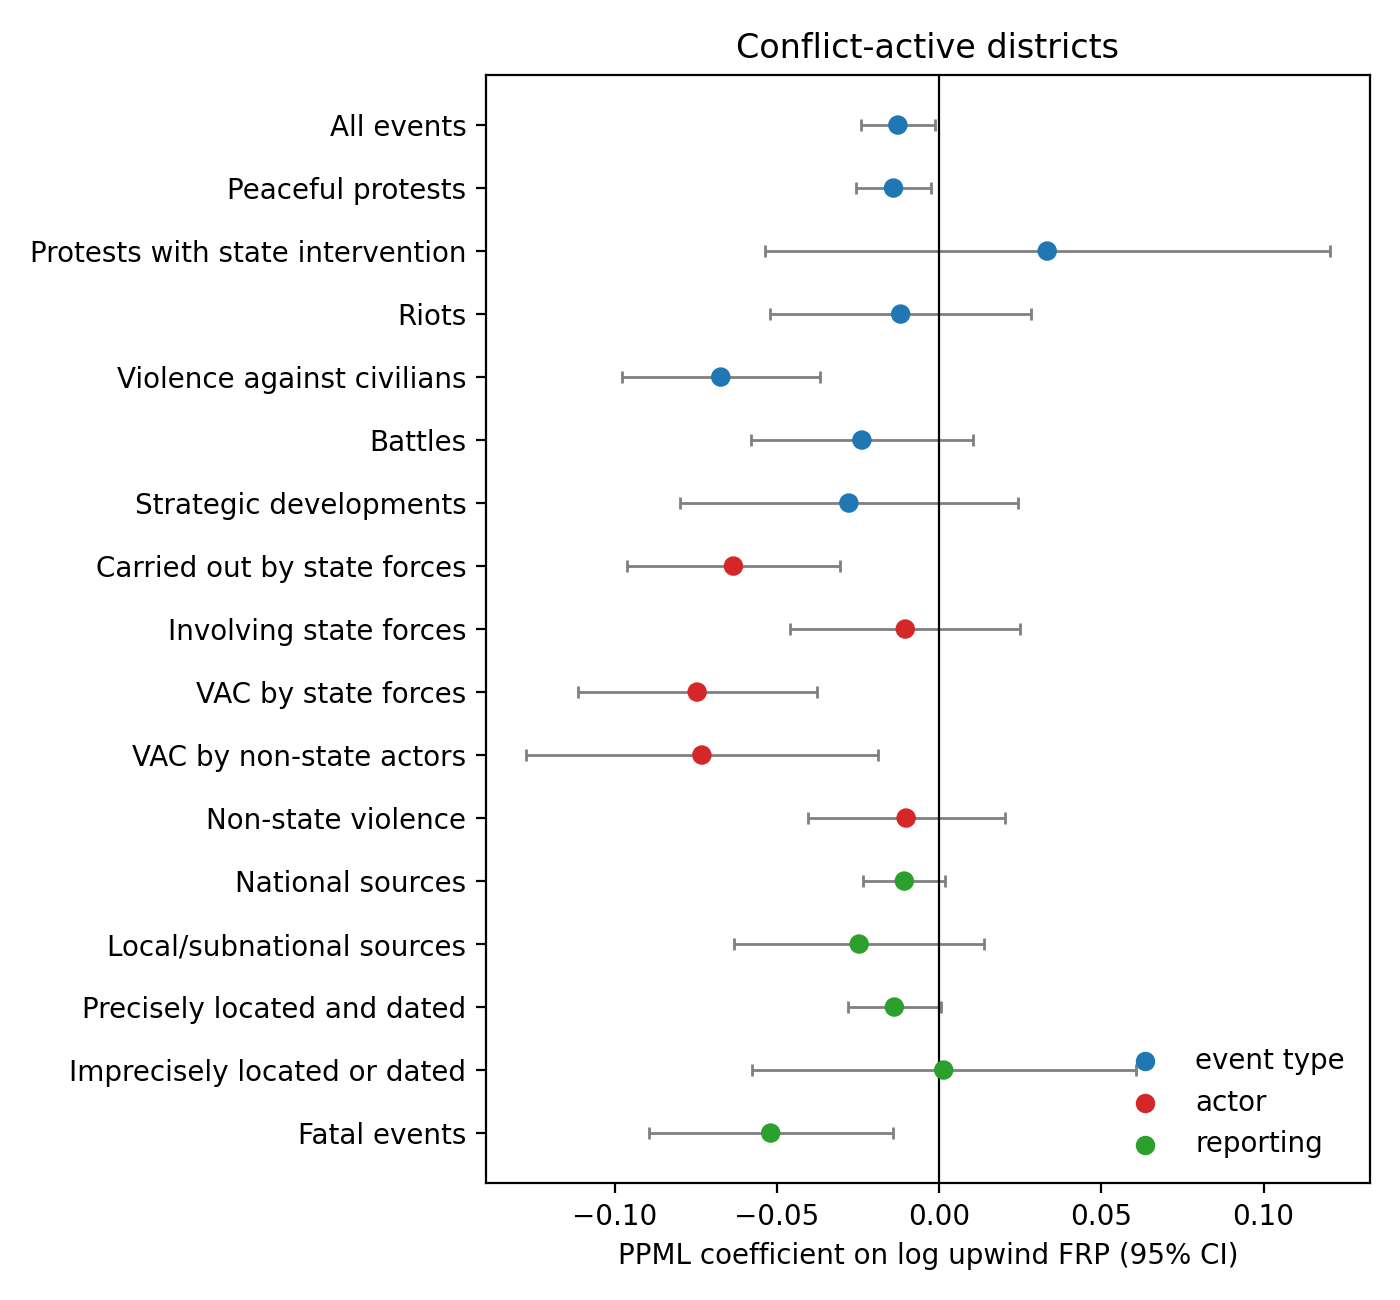
\includegraphics[width=0.75\textwidth]{figures/mechanisms_coefplot.png}
\caption{Proportional (PPML) effects of upwind fire on conflict outcomes in conflict-active districts, with 95\% confidence intervals. See Table~\ref{tab:mechanisms} for definitions.}
\label{fig:mechanisms}
\end{figure}

The evidence favours state-capacity diversion over the other two explanations, though not exclusively. In proportional terms, the largest declines are in events carried out by state forces ($-6.3\%$ per log point, $p<0.001$) and in violence against civilians, about five times the proportional decline in peaceful protests ($-1.4\%$, $p=0.017$). Protests account for most of the decline in the \emph{number} of events because they are by far the most common event type, but they fall by a much smaller percentage. Non-state violence as a whole does not decline (riots and battles show no effect), although violence against civilians by non-state actors, mostly armed groups in Papua, falls by a similar percentage to that by state forces. Avoidance receives some support: in levels, the protest decline is concentrated in cities (the interaction with a \emph{kota} indicator is $-0.033$, $p=0.014$), but in proportional terms it does not differ detectably between cities and rural districts. Severe fire years (2015, 2019 and 2023) do not amplify the effect detectably, although the interaction for events carried out by state forces is negative and marginally significant in OLS ($-0.006$, $p=0.054$).

The reporting explanation fits the data poorly. Events reported by national sources fall by a similar proportion to all events, events with imprecise locations or dates do not fall at all, and fatal events, the high-salience events least likely to go unreported, fall by about 5\% per log point ($p=0.007$), four times the proportional decline in all events. If haze reduced reporting, the opposite ordering would be expected. This does not rule out every form of reporting bias, but it is hard to reconcile with a decline driven by thinner coverage.

Finally, I test whether conflict is displaced rather than averted. If haze only postponed conflict, the months after exposure would show a rebound. Adding the second and third lags of upwind fire to the reduced form shows no rebound in all events: every lag coefficient is negative, and the cumulative effect over four months is $-0.037$ ($p=0.030$), larger than the contemporaneous effect alone. For events carried out by state forces, the one-month lag is positive ($+0.006$), consistent with the rebound in violence against civilians documented in Appendix Section~\ref{sec:fulliv}, but the cumulative effect remains negative. If conflict were displaced across space, a district's conflict would rise when its neighbours receive upwind fire. Controlling for a district's own exposure, the mean upwind fire of contiguous districts has a positive but insignificant coefficient ($+0.026$, $p=0.27$). Because own and neighbour exposure are highly correlated (0.88), this test has little power, and spatial displacement cannot be ruled out.

\subsection{Smoke or fire response? Same-province and other-province fire}
\label{sec:province}

The tests in Section~\ref{sec:mechanisms} distinguish among explanations by the type of event that declines, but they share one gap. Upwind fire often burns in other districts, so it is not obvious why it should draw on the security forces of the district that receives the smoke. Indonesia's fire-response arrangements suggest a sharper test. Fire task forces are organized by province, with the provincial military commander and police chief as deputy commanders \citep{inpres3_2020}, so fires in a district's own province draw on its security forces, whereas fires in another province reach the district only as smoke. If the decline in state violence reflects the diversion of security forces, it should respond mainly to same-province fire. If it reflects smoke, the source province should not matter.

I rebuild the upwind instrument exactly as in Section~\ref{sec:empirical}, but assign each upwind fire's FRP to a same-province or an other-province component according to the province in which it burns. The rebuilt total reproduces the original instrument on all 60,125 district-months. Same-province fires account for 54\% of upwind FRP, and the two components are only weakly correlated (0.23), so their effects can be estimated separately. Table~\ref{tab:province} reports the reduced form with both components and their one-month lags in the conflict-active subsample, and Figure~\ref{fig:province} plots the PPML coefficients.

\begin{table}[htbp]
\centering
\caption{Same-province and other-province upwind fire (conflict-active districts)}
\label{tab:province}
\resizebox{\textwidth}{!}{%
\begin{tabular}{lcccccc}
\toprule
 & \multicolumn{2}{c}{Same-province upwind fire} & \multicolumn{2}{c}{Other-province upwind fire} & Equality & \\
\cmidrule(lr){2-3}\cmidrule(lr){4-5}
Outcome & PPML coef. (SE) & $p$ & PPML coef. (SE) & $p$ & $p$-value & OLS equality $p$ \\
\midrule
All events & $-0.004$ (0.008) & 0.614 & $-0.013$ (0.005) & 0.011 & 0.347 & 0.237 \\
Peaceful protests & $-0.003$ (0.007) & 0.718 & $-0.018$ (0.005) & 0.001 & 0.078 & 0.064 \\
Carried out by state forces & $-0.045$ (0.017) & 0.009 & $-0.038$ (0.043) & 0.377 & 0.880 & 0.498 \\
Violence against civilians & $-0.064$ (0.016) & $<0.001$ & $-0.028$ (0.035) & 0.413 & 0.363 & 0.330 \\
VAC by state forces & $-0.068$ (0.017) & $<0.001$ & $-0.048$ (0.047) & 0.308 & 0.702 & 0.434 \\
Non-state violence & $-0.001$ (0.025) & 0.961 & $+0.005$ (0.019) & 0.796 & 0.875 & 0.857 \\
\bottomrule
\end{tabular}}
\begin{minipage}{0.95\textwidth}
\footnotesize \textit{Notes:} Reduced form with log same-province and log other-province upwind FRP and the one-month lag of each, district and year-month fixed effects, and standard errors clustered by province; 85 conflict-active districts. Coefficients are on the contemporaneous components. ``Equality'' tests that the two contemporaneous coefficients are equal. Upwind fire is defined as in Section~\ref{sec:empirical}; each fire is assigned to the province of the district in which it burns. Source: \texttt{analysis/state-capacity-province.ipynb}.
\end{minipage}
\end{table}

\begin{figure}[htbp]
\centering
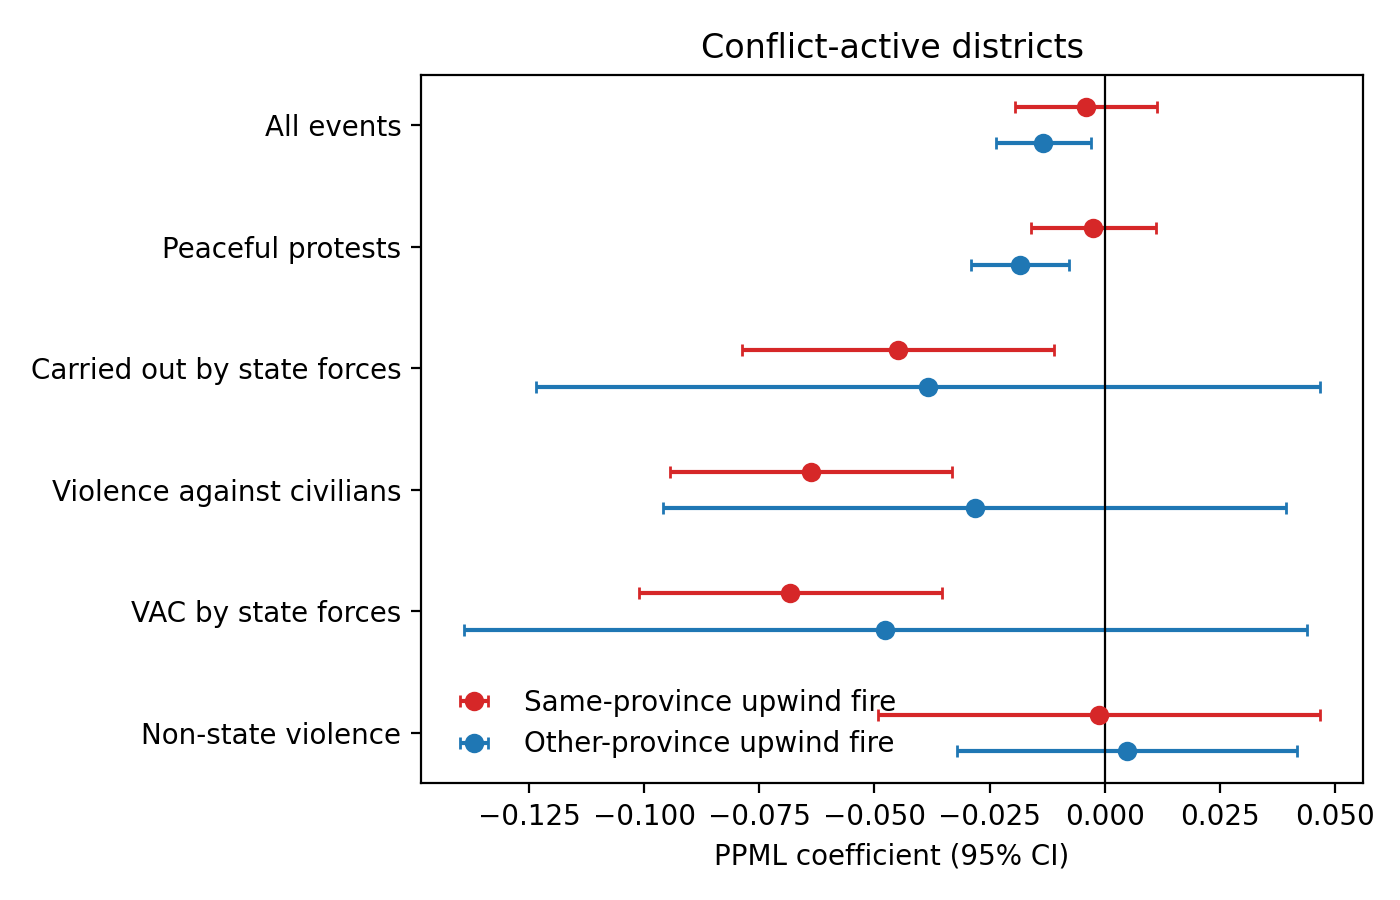
\includegraphics[width=0.75\textwidth]{figures/province_split_coefplot.png}
\caption{Proportional (PPML) effects of same-province and other-province upwind fire in conflict-active districts, with 95\% confidence intervals.}
\label{fig:province}
\end{figure}

The two kinds of event respond to different fires. The decline in peaceful protests comes from other-province fire ($-1.8\%$ per log point, $p=0.001$), while same-province fire has no detectable effect on protests ($-0.3\%$, $p=0.72$); the difference is marginally significant ($p=0.078$). Because fires in another province cannot draw on the district's security forces, this decline is best explained by the smoke itself, which makes it the cleanest evidence of a pollution channel in this paper. Events carried out by state forces, by contrast, fall significantly only with same-province fire ($-4.5\%$, $p=0.009$), as does violence against civilians by state forces ($-6.8\%$, $p<0.001$). The other-province estimates for these outcomes are similar in size but far less precise, so I cannot reject that the two components have equal effects ($p=0.88$ and $p=0.70$). The test therefore supports a smoke channel for protests more firmly than it supports a fire-response channel for state violence.

Two limitations apply. First, same-province fires are on average closer to the district (the correlation between the same-province component and fire within 150\,km is 0.79), so the contrast is partly a contrast between near and far fires. Splitting each component further by distance leaves too little independent variation: the resulting estimates are imprecise and change sign between distance bands. Second, a province-level fire response could also involve security forces from neighbouring provinces during the largest fires, which would blur the contrast. With these caveats, the results suggest two channels: smoke reduces protests, and the diversion of security forces to fire response plausibly reduces state violence.

\subsection{Additional robustness and specification checks}
\label{sec:robustness-summary}

I subject the results above to a series of additional checks. The location-precision check is reported here in full; each of the others is summarized briefly here and reported in full, with complete tables and discussion, in Appendix Section~\ref{sec:appendixrobustness}.

\paragraph{Poisson IV control function.} Following \citet{lu2023fish}, I re-estimate the full-sample relationship using a Poisson IV control-function approach \citep{terzabasurathouz2008} designed for severely zero-inflated count data. Unlike the baseline linear IV, the Poisson model finds a significant negative full-sample effect on \texttt{events} ($-0.040$, $p=0.013$), although its control-function residual is also significant ($p=0.038$), signaling remaining endogeneity; for \texttt{pv\_events}, neither the effect ($p=0.732$) nor the residual ($p=0.470$) is significant. The full-sample null for all events in Table~\ref{tab:mainiv} therefore depends on the linear specification (Appendix Table~\ref{tab:poisson}).

\paragraph{Conflict-related fatalities.} I do not find robust evidence that fire exposure affects conflict-related fatalities. Linear IV estimates are consistently negative but imprecise ($p$ between 0.089 and 0.177), and the one specification that yields a significant effect (a Poisson control function) shows clear signs of residual endogeneity and relies on a severely restricted, non-representative sample (Appendix Table~\ref{tab:fatalities}).

\paragraph{Exclusion restriction and inference.} I implement a placebo test that replaces each district's upwind instrument with a randomly-assigned, implausibly distant ($\geq 500$\,km) district's instrument, and find it is small, wrong-signed, and statistically insignificant, supporting the exclusion restriction. I also add a province $\times$ calendar-month fixed effect to absorb shared regional seasonal fire cycles, and compute Conley spatial-correlation standard errors that allow residual correlation across province boundaries. Under these three checks, the all-events and Riots/VAC results in conflict-active districts remain significant at the 5\% level, as does violence against civilians on its own (but see the regional-shocks and weak-instrument checks below); the political-violence result survives the seasonal fixed effect but not Conley standard errors ($p \approx 0.25$), and the protest result survives neither. With the seasonal fixed effect, the instrument is weak in the conflict-active subsample (effective $F = 10.5$), so those estimates should be read with caution (Appendix Tables~\ref{tab:placebo}--\ref{tab:conley}).

\paragraph{Location precision.} Conflict events are assigned to districts by their coordinates, and ACLED reports how precisely each event is located. For 109 events (0.5\% of the sample), only a larger region is known, so ACLED places them at that region's centroid or capital, where they may fall in the wrong district. Dropping these events leaves the results essentially unchanged: in the $\tau \geq 30\%$ subsample, the all-events estimate is $-0.178$ ($p=0.001$), Riots/VAC $-0.047$ ($p=0.028$), and political violence $-0.044$ ($p=0.065$), and the full-panel estimates remain small and insignificant.

\paragraph{Regional shocks and the district's own fires.} Two further checks target the exclusion restriction directly (Appendix Section~\ref{sec:regional}). First, province $\times$ year-month fixed effects absorb any shock common to a province in a given month, such as a regional drought. With them, the instrument is weak in the full panel (effective $F = 21.2$) and has essentially no power in the $\tau \geq 30\%$ subsample ($F = 1.9$), so this check cannot confirm or reject the result; the reduced-form point estimate is nearly unchanged ($-0.028$ vs.\ $-0.026$) but imprecise ($p=0.19$). Second, the upwind cone begins at the district centroid and so includes some fires inside the district itself (4.9\% of upwind FRP). Excluding them leaves the reduced form at $\tau \geq 30\%$ unchanged ($-0.029$, $p=0.004$), but it weakens the first stage in that subsample (effective $F = 9.5$), which suggests that much of the first stage's strength there came from the district's own fires. The IV estimates then become larger and less precise (all events $-0.346$, $p=0.018$). Because this first stage is below the conventional threshold of 10, I also report the Anderson--Rubin test, which rejects a zero effect on all events ($p=0.023$).

\paragraph{Local weather controls.} Drought raises fire activity and could also affect conflict directly through income, and neither the year-month nor the province $\times$ calendar-month fixed effects absorb an unusually dry or hot month in a particular district. I add ERA5 district-month total precipitation and 2\,m temperature, each with a one-month lag, as controls in both stages (Appendix Section~\ref{sec:weather}). Upwind fire is clearly related to weather (its correlation with precipitation is $-0.36$), but the reduced form at $\tau \geq 30\%$ is unchanged ($-0.026$, $p=0.002$, vs.\ $-0.026$, $p=0.002$ at baseline), as are its Riots/VAC and violence-against-civilians components. Because weather explains part of local fire intensity, the first stage weakens (effective $F = 15.6$, just above the 20\%-bias critical value of 15.1), and the IV coefficients grow (all events $-0.258$, $p=0.001$). Adding province $\times$ calendar-month fixed effects on top of the weather controls leaves the reduced form at $-0.026$ ($p=0.013$).

\paragraph{Weak-instrument-robust inference.} Several specifications above have weak first stages, where conventional 2SLS $p$-values are unreliable. The Anderson--Rubin test of a zero effect remains valid however weak the instrument is: it is a joint test that both instrument coefficients in the reduced form are zero. At $\tau \geq 30\%$, it rejects a zero effect on all events at baseline ($p=0.012$), with weather controls ($p=0.006$), and with weather controls and province $\times$ calendar-month fixed effects ($p=0.029$), but not with province $\times$ year-month fixed effects ($p=0.38$). Violence against civilians gives similar results ($p=0.024$ at baseline). Political violence ($p=0.16$) and Riots/VAC ($p=0.066$) are weaker than their 2SLS $p$-values suggest (Appendix Table~\ref{tab:ar}). With the instrument that excludes the district's own fires (effective $F = 9.5$), the test rejects a zero effect on all events ($p=0.023$) and violence against civilians ($p=0.007$).

\paragraph{Fully-instrumented distributed-lag IV.} The main specifications instrument only the contemporaneous treatment because \texttt{pyfixest} supports a single endogenous regressor, leaving the one-month lag as an uninstrumented control. Instrumenting both simultaneously leaves the conflict-active and event-type results unchanged in sign and significance (all events $-0.141$, $p=0.012$; Riots/VAC $-0.068$, $p<0.001$), but reveals that the full-panel null is not uniform: both all events ($-0.015$, $p=0.046$) and political-violence events ($-0.006$, $p=0.026$) show significant negative effects once the lag is properly instrumented, alongside positive lagged effects suggestive of a short-run disruption followed by a partial rebound (Appendix Table~\ref{tab:fulliv}). In the reduced form, however, longer lags show no rebound in all events (Section~\ref{sec:mechanisms}).


\paragraph{Placebo in time: leads of the instrument.} Next month's upwind fire cannot cause this month's conflict, so if it predicted conflict, the instrument would be picking up seasonal or regional trends rather than smoke exposure. Adding the one-month lead of the instrument to the reduced form, the lead coefficient for all events in the conflict-active subsample is essentially zero ($-0.0002$, $p=0.985$), no outcome has a lead coefficient with $p<0.25$ in either sample, and the contemporaneous coefficient is unchanged ($-0.0257$ without the lead, $-0.0256$ with it, $p=0.001$). Results are in Appendix Table~\ref{tab:idchecks}.

\paragraph{The 2018--2025 sample.} ACLED's coverage of Indonesia roughly triples in 2018 (333 events in 2017, 1,092 in 2018). If reporting improved unevenly across regions, the early years could distort the estimates. Restricting to 2018--2025 strengthens the results: in the same 85 conflict-active districts, the reduced form is $-0.036$ ($p=0.003$; effective $F = 25.5$; Anderson--Rubin $p=0.015$), and re-selecting conflict-active districts on their 2018--2025 event shares retains all 85 and adds 32 more, with a reduced form of $-0.030$ ($p=0.002$). In the full 2018--2025 panel, the Anderson--Rubin test rejects a zero effect for all four outcomes ($p$ between 0.006 and 0.048), even though the full-panel 2SLS estimates remain imprecise (Appendix Table~\ref{tab:idchecks}).

\paragraph{Multiple testing.} I test four outcomes. Sharpened $q$-values \citep{benjamini2006adaptive,anderson2008multiple}, which control the false discovery rate across the four, leave the all-events result significant in the conflict-active subsample in the reduced form ($q=0.009$; Bonferroni-adjusted $p=0.009$), in 2SLS ($q=0.002$), and under the Anderson--Rubin test ($q=0.050$). Violence against civilians is significant at the 5\% level under 2SLS ($q=0.027$) and the Anderson--Rubin test ($q=0.050$), while political violence remains marginal (Anderson--Rubin $q=0.090$). These results support the paper's reading that the all-events and violence-against-civilians results are robust and the political-violence result is suggestive.

\subsection{Is the conflict-active cutoff driving the result?}
\label{sec:propensity}

The heterogeneity result in Section~\ref{sec:active} depends on a cutoff ($\tau \geq 30\%$) that was not chosen in advance, and on an activity share measured over the same months used for estimation. To address both concerns, I measure each district's conflict propensity before the estimation window, as the share of months in 2015--2017 with any ACLED event, and estimate on 2018--2025 only. Because ACLED's early coverage of Indonesia is sparse, 52\% of districts have no events in 2015--2017, so I group districts by the number of months with any event in that period (0, 1, 2--5, and 6 or more) and estimate the reduced form separately in each group. As a second measure that keeps the full sample, I compute each district-year's propensity from all \emph{other} years (leave-one-year-out) and split districts into quintiles of its average.

\begin{figure}[H]
\centering
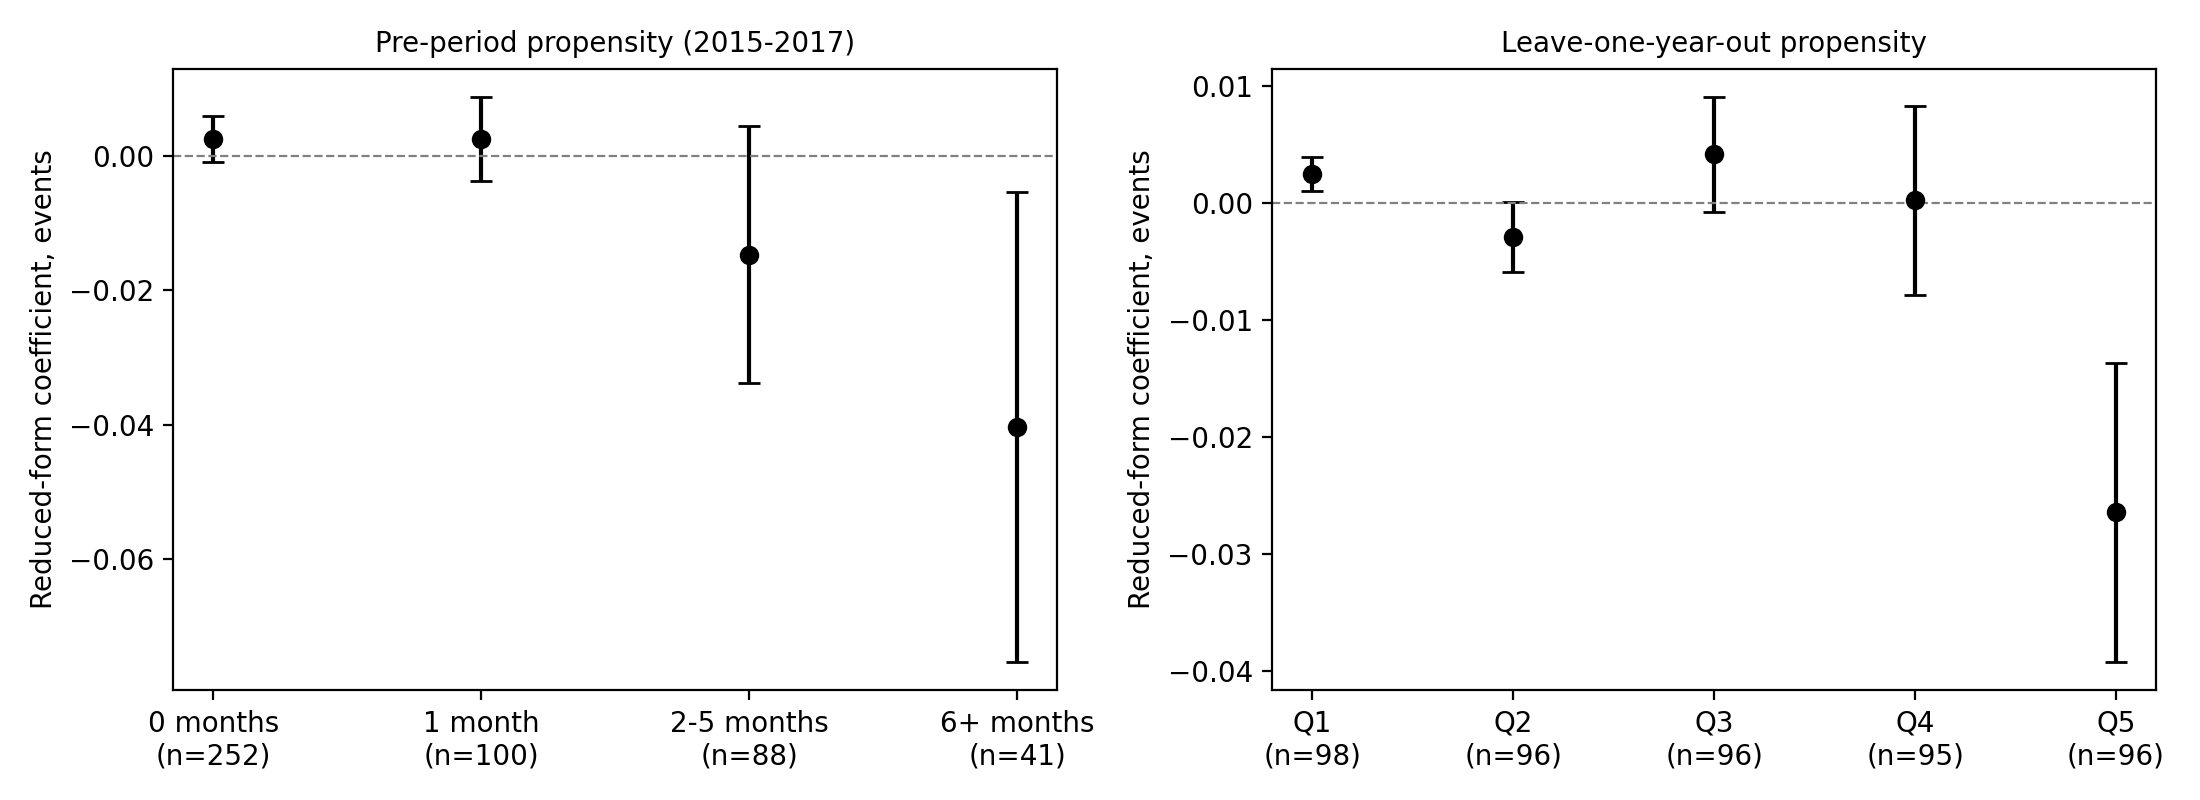
\includegraphics[width=\textwidth]{figures/conflict_propensity_bins.png}
\caption{Reduced-form effect of upwind fire by prior conflict propensity}
\label{fig:propensity}
\begin{minipage}{0.95\textwidth}
\vspace{4pt}
\footnotesize \emph{Notes:} Each point is the coefficient on contemporaneous log upwind FRP in a reduced-form regression of monthly conflict events on contemporaneous and lagged log upwind FRP, estimated separately for each group of districts, with district and year-month fixed effects; bars are 95\% confidence intervals from province-clustered standard errors. Left: districts grouped by the number of months in 2015--2017 with any ACLED event, estimated on 2018--2025. Right: quintiles of leave-one-year-out conflict propensity averaged within district, estimated on 2015--2025. Computed in \texttt{analysis/conflict-propensity.ipynb}.
\end{minipage}
\end{figure}

Figure~\ref{fig:propensity} shows that the effect is a gradient rather than an artifact of the cutoff. In districts with no prior conflict, or a single month of it, the reduced form is close to zero ($+0.003$ in both groups); it turns negative for districts with two to five months ($-0.015$, $p=0.14$) and is largest for the 41 districts with six or more ($-0.040$, $p=0.037$). The leave-one-year-out measure gives the same picture: only the top quintile is clearly negative ($-0.026$, $p<0.001$), matching the $\tau \geq 30\%$ estimate. In a linear specification that interacts the instrument with pre-period propensity, every interaction coefficient is negative; the joint test of the interaction terms rejects for political violence ($p=0.017$), Riots/VAC ($p=0.005$), and violence against civilians ($p=0.023$), but not for all events ($p=0.16$).

A Poisson version of the same interaction, which measures proportional rather than absolute effects, finds no gradient: the effect of upwind fire on all events is about $-1\%$ per log point regardless of propensity (main effect $p=0.11$; interaction $p=0.60$). The most consistent reading of these results is that upwind fire reduces conflict by a similar small percentage in all districts, and that this is only detectable in event counts where conflict is common enough for the percentage to be measurable. This also accounts for the full-sample null without requiring a mechanism specific to conflict-prone districts. It does mean that the results do not show that conflict-prone districts respond more strongly in proportional terms.

\subsection{Instrumenting pollution directly}
\label{sec:pollution}

The IV estimates in Sections~\ref{sec:active}--\ref{sec:fourway} instrument the district's own fire intensity, which, as Section~\ref{sec:estimand} explains, conflicts with the proposed smoke mechanism. Here I instead instrument a direct measure of air pollution. I use monthly surface PM2.5 from the MERRA-2 aerosol reanalysis (product M2TMNXAER; \citealp{gelaro2017merra}), constructed from its surface mass concentrations of dust and sea salt below 2.5\,$\mu$m, organic carbon, black carbon, and sulfate, following \citet{buchard2016}, and, as a second measure, total aerosol optical depth at 550\,nm. The MERRA-2 grid is $0.5^{\circ} \times 0.625^{\circ}$; each district is assigned the mean of the grid cells whose centres fall inside it, and districts that contain no cell centre are assigned the nearest cell. District-month PM2.5 averages 11.4\,$\mu$g/m$^3$, peaks in the September--October haze season, and reaches 239\,$\mu$g/m$^3$ during the 2019 fires. The specification mirrors Eq.~\eqref{eq:secondstage}, with log PM2.5 as the endogenous variable, its one-month lag as a control, and the same instruments, fixed effects and clustering. This IV identifies the effect of pollution under the exclusion restriction that upwind fire affects conflict only through the pollution it carries, which is the mechanism the paper proposes. A version that also controls for the district's own fire intensity (log FRP and its lag) guards against upwind fire acting through correlated local burning.

\begin{table}[H]
\centering
\caption{Instrumenting surface PM2.5 with upwind fire}
\label{tab:pollution}
\resizebox{\textwidth}{!}{%
\begin{tabular}{lcccc}
\toprule
 & Full panel & $\tau \geq 30\%$ & $\tau \geq 30\%$, 2018+ & $\tau \geq 30\%$, + own fire \\
\midrule
All events                 & $-0.079$ [0.304; AR 0.074] & $-1.227^{***}$ [0.005; AR 0.004] & $-1.683^{***}$ [0.005; AR 0.005] & $-1.071^{**}$ [0.025; AR 0.023] \\
Political violence         & $-0.023$ [0.277; AR 0.021] & $-0.339^{*}$ [0.062; AR 0.154] & $-0.529^{*}$ [0.064; AR 0.108] & $-0.394$ [0.128; AR 0.169] \\
Riots/VAC                  & $-0.026$ [0.242; AR 0.027] & $-0.372^{**}$ [0.032; AR 0.086] & $-0.491^{**}$ [0.031; AR 0.063] & $-0.430^{*}$ [0.083; AR 0.083] \\
Violence against civilians & $-0.023$ [0.147; AR 0.058] & $-0.258^{*}$ [0.051; AR 0.036] & $-0.348^{*}$ [0.054; AR 0.008] & $-0.306^{*}$ [0.087; AR 0.029] \\
\midrule
First stage (log upwind FRP) & $0.028^{***}$ & $0.021^{***}$ & $0.020^{***}$ & $0.019^{***}$ \\
Effective $F$ & 41.1 & 25.7 & 19.3 & 25.7 \\
Districts & 481 & 85 & 85 & 85 \\
\bottomrule
\end{tabular}%
}
\begin{minipage}{0.95\textwidth}
\vspace{4pt}
\footnotesize \emph{Notes:} Each cell reports the 2SLS coefficient on instrumented log PM2.5 (MERRA-2) in a regression of monthly event counts on log PM2.5 and its lag, with log PM2.5 instrumented by contemporaneous and lagged log upwind FRP; brackets give the conventional $p$-value and the Anderson--Rubin $p$-value. The last column adds the district's own log FRP and its lag as controls. District and year-month fixed effects; standard errors clustered by province. $^{***}p<0.01$, $^{**}p<0.05$, $^{*}p<0.1$. Computed in \texttt{analysis/pollution-iv.ipynb}.
\end{minipage}
\end{table}

Table~\ref{tab:pollution} reports the results. The first stage is strong: upwind fire significantly raises district PM2.5 in every sample, with effective $F$ between 19 and 48. In the conflict-active subsample, instrumented PM2.5 reduces conflict events ($-1.23$, Anderson--Rubin $p=0.004$), so a 10\% increase in PM2.5 reduces events by 0.12 per district-month, or 8.4\% of the subsample mean. The estimate is larger on 2018--2025 and changes little when the district's own fire is controlled for ($-1.07$, Anderson--Rubin $p=0.023$), so it does not reflect local burning. The event-type pattern matches Section~\ref{sec:eventtype}: violence against civilians is robust to weak-instrument inference (Anderson--Rubin $p=0.036$), while political violence is not ($p=0.15$). MERRA-2 aerosol optical depth gives the same signs and similar Anderson--Rubin $p$-values (all events $p=0.007$ in the conflict-active subsample), with a weaker first stage (effective $F = 16.1$). In the full panel, the 2SLS estimates are imprecise, but the Anderson--Rubin test rejects a zero effect for political violence ($p=0.021$) and Riots/VAC ($p=0.027$), consistent with the proportional-effect reading in Section~\ref{sec:propensity}.

Two qualifications apply. First, MERRA-2 is a reanalysis: it assimilates satellite aerosol optical depth, but its biomass-burning emissions are derived from satellite fire detections, so its PM2.5 is partly built from fire data of the kind the instrument uses. This does not invalidate the instrument, whose exogeneity comes from wind direction, but it means the endogenous variable is a modelled rather than a measured pollution exposure. Second, the grid is coarse relative to districts: 243 of 502 districts contain no grid-cell centre and take the nearest cell, so their pollution is measured with additional error. Classical measurement error in the endogenous variable does not bias 2SLS, but non-classical error could, and the large implied elasticity (about $-0.9$) should be read with that in mind; I emphasize the sign and significance over the exact magnitude.

\paragraph{Districts containing their own grid point.} To assess the second concern, I re-estimate the pollution IV only on the 259 districts that contain at least one grid-cell centre. This check is not informative in the conflict-active subsample. Conflict-active districts are disproportionately small cities (18 of the 85 are \emph{kota}, none of which contains a grid point), so only 25 of the 85 remain, and the first stage falls to an effective $F$ of 6.7. The point estimates remain negative (all events $-0.30$, violence against civilians $-0.42$) but are imprecise (Anderson--Rubin $p$ between 0.24 and 0.41). The loss of precision reflects the smaller sample rather than the pollution measure: the reduced form, which does not use MERRA-2, is also imprecise in these 25 districts ($-0.011$, $p=0.58$), while it is negative and significant in the 60 conflict-active districts that use the nearest cell ($-0.030$, $p=0.022$). In the 249 full-panel districts with their own grid point, the first stage is strong (effective $F = 49.0$), but the 2SLS estimates are close to zero, and the Anderson--Rubin test rejects for political violence ($p=0.027$) and Riots/VAC ($p=0.017$) without a clear sign. These results neither confirm nor refute that measurement error in the fallback districts drives the pollution estimates (Appendix Table~\ref{tab:owngrid}).

\paragraph{Satellite aerosol optical depth.} To address both qualifications, I construct an observed pollution measure: aerosol optical depth at 550\,nm from the MODIS MAIAC algorithm \citep{lyapustin2018maiac}, using its daily 0.05$^{\circ}$ (about 5\,km) gridded product (MCD19A2CMG, Terra and Aqua combined). At this resolution all but 4 of 502 districts contain their own pixels (median 62 per district). District-month AOD is the mean over all valid pixel-days; because retrievals are missing under cloud, on average only 24\% of pixel-days are valid, ranging from 12\% in January to 36\% in July. Monthly MAIAC AOD is correlated with MERRA-2 AOD (0.70 in logs) and PM2.5 (0.64), and it peaks in the September--October haze season.

The MAIAC first stage, however, is weak. Upwind fire does not significantly predict log MAIAC AOD in the full panel ($+0.002$, $p=0.46$; effective $F = 8.5$) or the conflict-active subsample ($+0.005$, $p=0.28$; effective $F = 4.2$), whereas on exactly the same district-months it strongly predicts MERRA-2 AOD ($+0.017$, $p=0.001$) and PM2.5 ($+0.028$, $p<0.001$). Restricting to district-months with at least 20\% valid coverage yields a small positive full-panel response ($+0.008$, $p=0.049$). Two explanations are consistent with this. First, the satellite record is selected on clear skies: retrieval coverage is positively correlated with upwind fire (0.24), because the dry season brings both clearer skies and more fires, and thick smoke is often flagged as cloud, so the smokiest days are the most likely to be missing from monthly MAIAC means. Second, MERRA-2's fire-emission inputs are derived from satellite fire detections, so part of its first stage may be mechanical. I cannot distinguish these explanations with monthly data.

Because the first stage is weak, the MAIAC 2SLS estimates are uninformative (Appendix Table~\ref{tab:maiac}). The Anderson--Rubin test, which remains valid, rejects a zero effect on all events in the conflict-active subsample ($p=0.005$), but with almost no first stage this rejection reflects the reduced-form relationship between upwind fire and conflict rather than evidence about pollution. In the full panel, the MAIAC 2SLS estimates are positive, opposite in sign to the MERRA-2 estimates, which is a further sign that this specification is not well identified. I therefore treat the MERRA-2 pollution IV as suggestive of a pollution channel, not as confirmation of it; the reduced form remains the paper's primary evidence.

\section{Discussion}
\label{sec:discussion}

The upwind-fire instrument is strong in the full panel (effective $F = 81.3$ in Table~\ref{tab:firststage}, and 75.7 in the distributed-lag specification), so the absence of an average effect in the baseline linear specification is not a symptom of weak identification. That null is fragile, however: the Poisson control function and the fully instrumented lag structure both find modest negative full-sample effects. Among districts where conflict is not a rare event, fire intensity has a large negative effect on conflict events, and this effect survives Conley standard errors and full instrumentation of the lag (and remains significant, with a weak instrument, under province $\times$ calendar-month fixed effects). The political-violence effect is less robust: it does not survive Conley standard errors. Within political violence, the effect operates through riots and violence against civilians, and the finer decomposition in Section~\ref{sec:fourway} shows that it comes mainly from violence against civilians rather than riots. Protests account for most of the decline in all events, but that estimate does not survive the stricter checks. The instrument is also weaker in the conflict-active subsample (effective $F = 26.4$, and $10.5$ with province $\times$ calendar-month fixed effects), so these estimates carry more weak-instrument risk than the full-panel ones.

\paragraph{Interpretation.} The mechanism tests in Sections~\ref{sec:mechanisms} and~\ref{sec:province} point to two channels. The first is smoke itself: protests decline, and the decline comes from fires in other provinces, which reach a district only as smoke and cannot draw on its security forces. The second is state capacity: in proportional terms, events carried out by state security forces fall about five times as much as peaceful protests, and they fall significantly only with fires in the district's own province. Fire emergencies in Indonesia draw on police and military personnel for firefighting, patrols and evacuation, which could reduce the routine operations in which security forces come into violent contact with civilians. The evidence for the first channel is firmer, because the province test cannot statistically separate same-province from other-province effects on state violence. Riots and battles do not respond to either. A reporting explanation fits poorly, since fatal events fall more than other events and imprecisely recorded events do not fall. Two qualifications apply. I do not observe deployments of security forces directly, and violence against civilians by non-state armed groups, mostly in Papua, also falls by a similar percentage, which a pure state-capacity explanation does not predict and which may reflect reduced operations by armed groups during haze. Whatever its precise channel, the direction of the effect is the opposite sign from much of the climate-conflict literature, which typically finds that adverse environmental shocks \emph{increase} conflict through resource scarcity or income-shock channels \citep{hsiang2013quantifying,burkehsiangmiguel2015,miguelsatyanathsergenti2004}. The contrast may reflect the very different time horizon at play: fire-driven haze is an acute, short-duration shock that operates through immediate logistical channels, such as the redeployment of security forces, rather than a persistent shock to income or resource availability that might generate grievance-based conflict over a longer horizon.

This result is also notable in light of the wind-instrumented pollution-and-behavior literature reviewed in Section~\ref{sec:litreview}. \citet{herrnstadt2021}, \citet{bondyrothsager2020}, and \citet{burkhardt2019} all find that short-run air pollution \emph{increases} violent crime, through either an aggression/irritant channel or a rational-choice discounting-of-punishment channel. The negative effect on conflict events documented here runs in the opposite direction. One reconciliation is that these are different outcomes operating through different channels. The pollution-crime literature studies individual aggressive or criminal acts that require neither coordination nor organizational capacity, whereas the ACLED events studied here are collective or organized actions: protests are carried out by crowds and, in this sample, violence against civilians mostly by state security forces and armed groups. Pollution could raise individual irritability and aggression while simultaneously reducing organized contention, if the organizations that carry it out, above all the security forces, are stretched by fire and haze response. The two findings need not be in tension, even though the outcomes move in opposite directions.

\paragraph{Caveats and next steps.} Several issues qualify the results above. The conflict-active sample restriction raises an obvious external-validity concern: the documented effect applies to districts where conflict is already a recurring phenomenon, so Section~\ref{sec:active} is best read as a heterogeneity analysis rather than a population-average one. The full-sample null is itself fragile, since the Poisson control function and the fully instrumented lag both find modest negative average effects. Inference is uneven across outcomes: the all-events, Riots/VAC, and violence-against-civilians results survive Conley standard errors and full instrumentation of the lag, and remain significant with province $\times$ calendar-month fixed effects (where the instrument is weak), although under the weak-instrument-robust Anderson--Rubin test only the all-events and violence-against-civilians results remain significant at the 5\% level; the political-violence result does not survive Conley standard errors, and the protest result, which accounts for most of the all-events decline, survives none of the stricter checks. The instrument is also weaker in the conflict-active subsample (effective $F = 26.4$), weak once province $\times$ calendar-month fixed effects are added ($10.5$) or the district's own fires are excluded from it ($9.5$), and uninformative with province $\times$ year-month fixed effects ($1.9$). The reduced form, which does not depend on first-stage strength, is the more reliable evidence in this subsample: it is stable at about $-0.03$ across these checks, although it is imprecise once province $\times$ year-month fixed effects remove most of the variation. Controlling for local rainfall and temperature, which could affect both fire activity and conflict, leaves the reduced form unchanged (Appendix Section~\ref{sec:weather}). The pollution IV in Section~\ref{sec:pollution} moves the identifying assumption closer to the proposed mechanism, but it relies on a coarse, modelled pollution measure whose fire emissions come from satellite fire detections; an observed measure, satellite aerosol optical depth, does not respond detectably to upwind fire, plausibly because cloud and thick smoke remove the haziest days from the satellite record. Daily data matching satellite retrievals to same-day conflict, or ground-based PM2.5 monitors, would be needed to settle whether upwind fire raises observed pollution in these districts. The gradient in Section~\ref{sec:propensity} replaces the conflict-active cutoff with a pre-determined measure, but in proportional terms the effect does not vary detectably with conflict propensity. Two further loose ends deserve dedicated follow-up: the positive lagged coefficient that emerges once the lag is properly instrumented (Appendix Section~\ref{sec:fulliv}) was not anticipated by the original design, although the reduced-form lag tests in Section~\ref{sec:mechanisms} find no rebound in all events; and although the tests in Section~\ref{sec:mechanisms} are hard to reconcile with a reporting explanation, external data on media coverage across high- and low-haze periods would be needed to rule it out fully.

\section{Future Research Directions}
\label{sec:future}

This paper opens several avenues for future work, beyond the immediate robustness checks noted in Section~\ref{sec:discussion}.

\paragraph{The lagged rebound pattern.} Appendix Section~\ref{sec:fulliv} finds that once the one-month lag is properly instrumented rather than entering as an uninstrumented control, its coefficient becomes large, positive, and often statistically significant, alongside a negative contemporaneous effect. The reduced-form tests in Section~\ref{sec:mechanisms} show that this does not amount to displacement over time for all events: with three lags of upwind fire, every lag coefficient is negative and the four-month cumulative effect is larger than the contemporaneous effect alone. A partial rebound appears only for events carried out by state forces, consistent with operations being postponed by a month. Longer lag structures and daily data would clarify the timing.

\paragraph{Direct evidence on security-force deployment and reporting.} The state-capacity interpretation rests on the composition of ACLED events rather than on direct observation of where security forces were deployed. Records of police and military participation in fire response, for example from Indonesia's national disaster management agency (BNPB) or provincial fire task forces, would allow a direct test of whether districts that send more personnel to fire response see larger declines in state-force events. Similarly, although the reporting tests in Section~\ref{sec:mechanisms} argue against a reporting explanation, external data on local media coverage during high- and low-haze periods would rule it out more fully.

\paragraph{Mechanism validation with finer-grained data.} Daily (rather than monthly) conflict and pollution data, for example ground-level PM2.5 or satellite aerosol optical depth merged with daily ACLED event timing, would allow a sharper test of whether protests and state violence drop specifically on high-haze days, and would help resolve whether the satellite pollution measure's weak response reflects missing retrievals on the haziest days.

\paragraph{Heterogeneity by El Ni\~{n}o phase.} Indonesian fire activity is strongly modulated by the El Ni\~{n}o--Southern Oscillation, with major haze episodes (2015, 2019, 2023) occurring during El Ni\~{n}o years. Section~\ref{sec:mechanisms} finds no detectable difference in the reduced-form effect in these years, but a simple year indicator is a coarse measure of fire-season severity. Interacting the effect with a continuous ENSO index, or with measures of the scale of each year's fire response, would test the state-capacity channel more directly, since that channel predicts larger effects when fire-response demands are greatest.

\paragraph{Alternative and complementary outcomes.} The analysis here focuses on conflict event counts. Incorporating economic outcomes (e.g., nighttime lights, mobility indices from cell-phone or satellite data, market activity) alongside conflict would help establish whether fire exposure also reduces economic activity, and whether reduced economic activity itself partially explains the drop in conflict events.

\paragraph{Spatial spillovers and displacement.} If haze suppresses conflict in one district, contention may be displaced to a neighboring, less-affected district rather than eliminated. The neighbor-exposure test in Section~\ref{sec:mechanisms} is inconclusive, because own and neighbor exposure are highly correlated. A spatial model that allows for cross-district spillovers in the instrumented treatment, for example a spatial-lag or SAR-2SLS specification as in \citet{lu2023fish}, would test for such displacement and provide a more accurate estimate of the aggregate (rather than purely local) effect.

\paragraph{Extending the sample period and out-of-sample validation.} The current panel runs through June 2025. As more recent VIIRS, ERA5, and ACLED data become available, extending the panel would increase power for the conflict-active subsample analysis and allow an out-of-sample test of whether the $\tau \geq 30\%$ threshold result documented in Table~\ref{tab:active} holds in years not used to select that threshold.

\paragraph{Cross-country comparison.} Indonesia is not the only country with recurring large-scale land-clearing fires (e.g., Brazil, parts of Sub-Saharan Africa). Replicating the upwind-instrument design in other settings would help establish whether the smoke and state-capacity channels suggested here are a general feature of fire-driven air pollution shocks or specific to Indonesia's political and climatic context.

\section{Conclusion}
\label{sec:conclusion}

Using a district-month panel for Indonesia and variation in fire activity upwind of each district, I find that wind-borne fire exposure reduces conflict where conflict is common. Across all districts the average effect is small and insignificant, but the effect grows with a district's conflict history measured before the estimation window, and in proportional terms it is similar across districts, which suggests a small percentage decline that is only measurable where conflict is frequent. The reduced-form result is unchanged when fires inside the district are excluded and when local rainfall and temperature are controlled for, and it survives spatially correlated standard errors, weak-instrument-robust inference, a placebo test using leads of the instrument, a later and better-covered sample, and a false-discovery-rate correction across outcomes.

The pattern of declines points to two channels. Protests fall with smoke from fires in other provinces, which cannot draw on local security forces, so this decline is best explained by smoke itself. Events carried out by state security forces fall about five times as much as protests in proportional terms, and significantly only with fires in the district's own province, consistent with security forces being diverted to fire response, although this contrast is not statistically decisive. Fatal events fall more than other events, which argues against reduced reporting, and conflict does not rebound in later months. Instrumenting reanalysis surface PM2.5 with upwind fire suggests that higher pollution reduces conflict, but satellite-observed aerosols do not respond detectably to upwind fire, so the pollution channel is not yet confirmed with observed data.

These results bring together two literatures that have largely run in parallel: work on climate and conflict, which typically finds that adverse environmental shocks increase conflict through resource-scarcity or income channels \citep{hsiang2013quantifying,burkehsiangmiguel2015}, and work using wind- and pollution-based designs, which finds that short-run air pollution increases individual aggression and crime \citep{herrnstadt2021,bondyrothsager2020,burkhardt2019}. The negative effect on collective and state-led contention documented here suggests that acute environmental shocks can reduce conflict both by discouraging collective action directly and by straining the operational capacity of the security forces, a combination that neither literature has, to my knowledge, examined directly.

\section*{Data Availability Statement}

All analysis code, including the panel-construction, instrument-construction, and estimation notebooks described throughout this paper, is available at \href{https://github.com/Hariaksha/wildfire-conflict}{github.com/Hariaksha/wildfire-conflict}. The conflict data (ACLED) and the processed wind, precipitation, and temperature data (ERA5) used in this paper are also hosted in that repository; the weather controls are constructed in \texttt{analysis/weather-controls.ipynb}, the pollution measures (MERRA-2 and MODIS MAIAC) and pollution IV in \texttt{analysis/pollution-iv.ipynb}, the conflict-propensity analysis in \texttt{analysis/conflict-propensity.ipynb}, and the lead, 2018--2025 and multiple-testing checks in \texttt{analysis/identification-checks.ipynb}. The processed district-month MERRA-2 PM2.5 and aerosol optical depth and MODIS MAIAC aerosol optical depth are also in the repository. The two largest raw inputs, fire detections and administrative boundaries, exceed standard GitHub file-size limits and are instead available directly from their original public sources:
\begin{itemize}
    \item \textbf{Fire detections:} NASA VIIRS active fire product (Suomi-NPP, 375\,m resolution), available via NASA FIRMS at \url{https://firms.modaps.eosdis.nasa.gov/download/}.
    \item \textbf{Administrative boundaries:} GADM v4.1 Indonesia boundaries (Level 2, kabupaten/kota), available at \url{https://gadm.org/download_country.html}.
    \item \textbf{Conflict events:} ACLED Indonesia data, available with registration at \url{https://acleddata.com}.
    \item \textbf{Wind fields:} ERA5 monthly averaged reanalysis on single levels \citep{hersbach2023era5}, available via the Copernicus Climate Data Store at \url{https://cds.climate.copernicus.eu/datasets/reanalysis-era5-single-levels-monthly-means} (DOI: \href{https://doi.org/10.24381/cds.f17050d7}{10.24381/cds.f17050d7}).
    \item \textbf{Pollution:} MERRA-2 monthly aerosol diagnostics, M2TMNXAER v5.12.4 \citep{gelaro2017merra}, available with a free NASA Earthdata account from the NASA GES DISC (DOI: \href{https://doi.org/10.5067/FH9A0MLJPC7N}{10.5067/FH9A0MLJPC7N}); and MODIS MAIAC aerosol optical depth, MCD19A2CMG v061 \citep{lyapustin2018maiac}, from NASA LP DAAC with the same account.
\end{itemize}
Replication of the full pipeline, from raw downloads through the figures and tables in this paper, requires retrieving the fire and boundary data from the sources above and placing them in the directory structure expected by the notebooks in the repository (documented in the repository's README). This paper contains modified Copernicus Climate Change Service information (2023); neither the European Commission nor ECMWF is responsible for any use that may be made of the Copernicus information or data it contains.

\clearpage
\appendix
\renewcommand{\thetable}{A\arabic{table}}
\setcounter{table}{0}
\renewcommand{\thefigure}{A\arabic{figure}}
\setcounter{figure}{0}

\section*{Appendix}

This appendix reports additional data description (Appendix~\ref{sec:appendixdata}), preliminary non-instrumented correlational evidence motivating the identification strategy in Section~\ref{sec:empirical} (Appendix~\ref{sec:preliminary}), and the complete robustness and specification checks summarized in Section~\ref{sec:robustness-summary} (Appendix~\ref{sec:appendixrobustness}).

\section{Additional Data Description}
\label{sec:appendixdata}

\begin{table}[H]
\centering
\caption{Summary statistics, district-month panel (Feb.\ 2015--Jun.\ 2025)}
\label{tab:sumstats}
\begin{tabular}{lcccc}
\toprule
Variable & Mean & SD & Zero share & N \\
\midrule
$\log(1+\text{FRP})$       & 2.045 & 2.244 & --     & 60{,}125 \\
events (all)               & 0.360 & 1.298 & 82.9\% & 60{,}125 \\
pv\_events (political violence) & 0.059 & 0.391 & 96.0\% & 60{,}125 \\
\bottomrule
\end{tabular}
\begin{minipage}{0.85\textwidth}
\vspace{4pt}
\footnotesize \emph{Notes:} Panel covers 481 districts $\times$ 125 months. ``Zero share'' is the fraction of district-month observations with a value of exactly zero.
\end{minipage}
\end{table}

\begin{figure}[H]
\centering
\includegraphics[width=0.85\textwidth]{figures/conflict_events_map.png}
\caption{\emph{All} ACLED conflict events recorded in Indonesia, February 2015--June 2025 ($n=21{,}653$). The map shows every recorded event; all of them are assigned to a GADM Level-2 district and enter the district-month panel (Section~\ref{sec:data}).}
\label{fig:conflictmap}
\end{figure}

\begin{figure}[H]
\centering
\includegraphics[width=0.85\textwidth]{figures/wildfire_events_map.png}
\caption{VIIRS wildfire detections in Indonesia, February 2015--June 2025 ($n=2{,}036{,}003$; vegetation fires only, type=0, confidence h/n). Color indicates $\log(1+\text{FRP})$.}
\label{fig:firemap}
\end{figure}

\section{Preliminary Correlational Evidence}
\label{sec:preliminary}

This appendix documents what a naive, non-instrumented approach finds, both to motivate the IV strategy used in the main text (Section~\ref{sec:empirical}) and to situate the paper's contribution relative to a simpler correlational analysis. In earlier exploratory work, I estimated a series of Poisson fixed-effects models regressing conflict outcomes on (uninstrumented) fire intensity at several different spatial and temporal resolutions, with no attempt to address the endogeneity of local fire activity.

Table~\ref{tab:prelim} summarizes five such specifications. The first models a province-week panel of population exposure on the (unlogged) count of local fire detections and its one-week lag; the second aggregates to province-month and uses log total FRP as the regressor for conflict event counts; the third and fourth estimate kabupaten-week and kecamatan-week panels of conflict events on log FRP with a 16-week distributed-lag structure; and the fifth repeats the kabupaten-week specification on a grid of equal-area cells rather than administrative units.

\begin{table}[H]
\centering
\caption{Preliminary Poisson FE models, uninstrumented fire intensity}
\label{tab:prelim}
\resizebox{\textwidth}{!}{%
\begin{tabular}{lccccc}
\toprule
Specification & Unit & Outcome & Regressor & Coef. (contemp.) & $p$-value \\
\midrule
Province-week        & province $\times$ week  & pop. exposure & $n$\_fires       & $-0.0002$ & $0.070$ \\
Province-month       & province $\times$ month & events        & log total FRP    & $0.0372$  & $0.535$ \\
Kabupaten-week        & district $\times$ week  & events        & log FRP          & $-0.0100$ & $0.631$ \\
Kecamatan-week        & sub-district $\times$ week & events    & log FRP          & $\approx 0.0000$ & $1.000$ \\
Equal-area grid-week  & $1^\circ$ cell $\times$ week & events  & log FRP          & $-0.0119$ & $0.187$ \\
\bottomrule
\end{tabular}%
}
\begin{minipage}{0.95\textwidth}
\vspace{4pt}
\footnotesize \emph{Notes:} All models include unit and time fixed effects and cluster-robust standard errors; the kabupaten-, kecamatan-, and grid-week specifications additionally include 16 weekly lags of log FRP (not shown). No instrumentation for fire intensity is used in any specification. ``Contemp.'' refers to the coefficient on the contemporaneous fire-intensity regressor.
\end{minipage}
\end{table}

The contemporaneous coefficient on fire intensity is statistically insignificant ($p > 0.05$) in every specification, and its sign is unstable across resolutions (negative in three of five, positive in one, and essentially zero in another). In the distributed-lag specifications (kabupaten-, kecamatan-, and grid-week), a handful of individual lag coefficients out of 17 are statistically significant at conventional levels, but these do not follow a consistent or interpretable temporal pattern and differ across specifications -- the signature of multiple testing under the null rather than a real dynamic effect.

Overall, these results suggest that a purely correlational approach, regressing conflict on local fire intensity however finely resolved spatially or temporally, does not reveal a stable relationship, whether because no such relationship exists or because local fire intensity is confounded with other local determinants of conflict. This motivated the instrumented design developed in Section~\ref{sec:empirical}, which (i) isolates plausibly exogenous variation in local fire exposure using the physical transport of smoke, and (ii) as shown in Section~\ref{sec:results}, reveals no robust average relationship, but a negative relationship within the subset of conflict-active districts once endogeneity and zero-inflation are addressed, most robustly for all conflict events and for violence against civilians.

\section{Additional Robustness Checks}
\label{sec:appendixrobustness}

This appendix reports, in full, seven of the eight additional robustness and specification checks summarized in Section~\ref{sec:robustness-summary} (the location-precision check is reported in full there): a Poisson IV control-function specification, an analysis of conflict-related fatalities, two checks of the instrument's exclusion restriction (a placebo test and a shared-seasonality test) plus Conley spatial-correlation standard errors, a fully-instrumented distributed-lag IV specification, two checks on regional shocks and on fires inside the district itself, controls for local rainfall and temperature, and weak-instrument-robust Anderson--Rubin tests.

\subsection{Robustness: Poisson IV control function}
\label{sec:poisson}

As a final robustness check on the full-sample null (Table~\ref{tab:mainiv}), I consider whether the linear IV specification is simply ill-suited to the severely zero-inflated count outcomes. \citet{lu2023fish}, who also study a conflict count, use a Poisson IV control-function estimator \citep{terzabasurathouz2008} as a robustness check on their 2SLS estimates. I implement the analogous two-step procedure on the full district panel:

\begin{enumerate}
    \item \textbf{Stage 1:} Regress $\text{logFRP}_{dt}$ on the excluded instruments $(\text{logZ}_{dt}, \text{logZ}_{d,t-1})$ \emph{and} the exogenous lag control $\text{logFRP}_{d,t-1}$, with district and year-month fixed effects, and compute the residual $\hat{v}_{dt} = \text{logFRP}_{dt} - \widehat{\text{logFRP}}_{dt}$. Including the exogenous lag control in the first stage (rather than only the excluded instruments) ensures $\hat{v}_{dt}$ is orthogonal to $\text{logFRP}_{d,t-1}$, as a correctly-specified two-stage residual inclusion estimator requires.
    \item \textbf{Stage 2:} Estimate a Poisson fixed-effects model of the conflict outcome on $\text{logFRP}_{dt}$, $\text{logFRP}_{d,t-1}$, and the control function $\hat{v}_{dt}$, with district and year-month fixed effects. A statistically significant coefficient on $\hat{v}_{dt}$ would indicate that $\text{logFRP}_{dt}$ is endogenous and that the Poisson estimate of its coefficient should be interpreted with caution; an insignificant coefficient indicates limited endogeneity bias.
\end{enumerate}

\begin{table}[H]
\centering
\caption{Poisson IV control function, full panel}
\label{tab:poisson}
\begin{tabular}{lcc}
\toprule
 & events & pv\_events \\
\midrule
$\text{logFRP}_{dt}$       & $-0.0403^{**}$ & $-0.0129$ \\
                            & (0.0163) & (0.0376) \\
                            & [$p=0.013$] & [$p=0.732$] \\
$\text{logFRP}_{d,t-1}$    & $0.0055$ & $-0.0008$ \\
                            & (0.0112) & (0.0186) \\
                            & [$p=0.625$] & [$p=0.967$] \\
$\hat{v}_{dt}$ (control function) & $0.0302^{**}$ & $0.0297$ \\
                            & (0.0146) & (0.0411) \\
                            & [$p=0.038$] & [$p=0.470$] \\
\midrule
District FE     & Yes & Yes \\
Year-month FE   & Yes & Yes \\
Observations     & 60{,}125 & 47{,}500 \\
\bottomrule
\end{tabular}
\begin{minipage}{0.85\textwidth}
\vspace{4pt}
\footnotesize \emph{Notes:} Stage 1 regresses $\text{logFRP}_{dt}$ on the excluded instruments and the exogenous lag control $\text{logFRP}_{d,t-1}$ (with district and year-month fixed effects); $\hat{v}_{dt}$ is the resulting residual. Stage 2 is a Poisson fixed-effects regression, with standard errors clustered by province in parentheses. These standard errors do not account for the estimation of $\hat{v}_{dt}$ in Stage 1, so they likely understate uncertainty; a bootstrap over both stages would correct this. The \texttt{pv\_events} model has fewer observations because the 101 districts that record no political-violence event over the sample period contribute nothing to the Poisson fixed-effects likelihood and are dropped (380 districts $\times$ 125 months $=$ 47{,}500); every district records at least one event of some type, so the \texttt{events} model retains all 60{,}125 observations. $^{***}p<0.01$, $^{**}p<0.05$, $^{*}p<0.1$.
\end{minipage}
\end{table}

For \texttt{pv\_events}, neither the Poisson coefficient on $\text{logFRP}_{dt}$ ($p=0.732$) nor the control-function residual ($p=0.470$) is significant, so the political-violence null carries over to the count-data specification. For \texttt{events}, however, the Poisson model finds a significant negative full-sample effect ($-0.040$, $p=0.013$), in the same direction as the conflict-active results, and the control-function residual is also significant ($+0.030$, $p=0.038$), indicating that endogeneity remains even after instrumenting. In \citet{lu2023fish}, the positive effects found with linear IV carry over to the Poisson control-function specification. Here, the full-sample null for all events is not robust to moving from a linear to a count-data specification; because these standard errors understate uncertainty and the residual signals remaining endogeneity, I read the Poisson \texttt{events} estimate as suggestive evidence of a modest negative average effect rather than as a precise estimate.

\subsection{Conflict severity: fatalities}
\label{sec:fatalities}

The outcomes considered so far (\texttt{events}, \texttt{pv\_events}) measure conflict \emph{intensity} in terms of event counts. A natural complementary outcome is conflict \emph{severity}: the number of fatalities ACLED records for each district-month, \texttt{fatalities}. This outcome is even more extremely zero-inflated than \texttt{events}: 98.9\% of district-months record zero fatalities, with a mean of 0.027 fatalities per district-month, so I report the same set of specifications used above: the full-panel linear IV (distributed-lag and contemporaneous-only), the $\tau \geq 30\%$ conflict-active subsample, and the Poisson IV control function. Table~\ref{tab:fatalities} reports the results.

\begin{table}[H]
\centering
\caption{Fatalities: IV estimates across specifications}
\label{tab:fatalities}
\resizebox{\textwidth}{!}{%
\begin{tabular}{lccc}
\toprule
Specification & $\text{logFRP}_{dt}$ & $\hat{v}_{dt}$ & Observations \\
\midrule
Full panel, distributed lags (IV-5)      & $-0.0230$ (0.0167) [$p=0.177$] & -- & 60{,}125 \\
Full panel, contemporaneous (IV-6)       & $-0.0138$ (0.0098) [$p=0.166$] & -- & 60{,}125 \\
Conflict-active, $\tau \geq 30\%$         & $-0.0653^{*}$ (0.0373) [$p=0.089$] & -- & 10{,}625 \\
Poisson IV control function (full panel) & $-0.9496^{**}$ (0.4257) [$p=0.026$] & $+0.8513^{**}$ (0.3490) [$p=0.015$] & 21{,}472 \\
\bottomrule
\end{tabular}%
}
\begin{minipage}{0.95\textwidth}
\vspace{4pt}
\footnotesize \emph{Notes:} ``Full panel, distributed lags'' and ``contemporaneous'' mirror IV-1/IV-3 in Table~\ref{tab:mainiv} but with \texttt{fatalities} as the outcome. ``Conflict-active'' mirrors the $\tau \geq 30\%$ row of Table~\ref{tab:active}. The Poisson IV control function mirrors Table~\ref{tab:poisson}; its observation count is far lower because the Poisson fixed-effects likelihood drops the 305 districts and 3 year-months that record no fatalities over the sample period (leaving 176 districts $\times$ 122 months $=$ 21{,}472). Standard errors clustered by province in parentheses. $^{***}p<0.01$, $^{**}p<0.05$, $^{*}p<0.1$.
\end{minipage}
\end{table}

The linear IV estimates for fatalities are qualitatively similar in sign to the \texttt{events} and \texttt{pv\_events} results: negative in all three linear specifications, including the $\tau \geq 30\%$ conflict-active subsample, where the point estimate ($-0.065$) is large relative to the mean, but none is significant at the 5\% level ($p$ between 0.089 and 0.177). This is unsurprising given that fatalities are roughly an order of magnitude rarer than events of any kind (98.9\% vs.\ 82.9\% zeros), so the linear IV likely lacks power to detect an effect of similar relative magnitude to the event-count results.

The Poisson IV control function tells a different, and more cautionary, story. Both $\text{logFRP}_{dt}$ ($-0.950$, $p=0.026$) and the control-function residual $\hat{v}_{dt}$ ($+0.851$, $p=0.015$) are significant at the 5\% level, and the residual is far larger than in the \texttt{events} and \texttt{pv\_events} Poisson models in Table~\ref{tab:poisson}. A significant $\hat{v}_{dt}$ indicates that $\text{logFRP}_{dt}$ is endogenous with respect to fatalities even after instrumenting, so the Poisson coefficient on $\text{logFRP}_{dt}$ in this specification should \emph{not} be read as a causal estimate. Compounding this, the sample used by \texttt{fepois} drops to 21{,}472 observations (36\% of the full panel), because the Poisson fixed-effects likelihood drops every district (305 of 481) and year-month (3 of 125) that records no fatalities over the sample period, which is common when 98.9\% of observations are zero. This non-random sample restriction further undermines a causal interpretation of the Poisson IV fatalities coefficient.

Altogether, I do not find robust evidence that wildfire exposure causally affects conflict-related fatalities: the linear IV estimates are suggestively negative but imprecise, and the one specification that returns a large, significant effect (Poisson IV control function) shows clear signs of residual endogeneity and a severely restricted, non-representative sample. This is itself an informative null: it suggests that the effect documented in Sections~\ref{sec:eventtype}--\ref{sec:fourway} operates primarily on the \emph{occurrence} of low-fatality events, rather than on the occurrence or severity of lethal violence, consistent with the absence of any effect on battles and remote violence in the event-type decompositions. A clean test of effects on fatalities would likely require a longer panel or a coarser unit of aggregation to overcome the extreme rarity of fatal events.

\subsection{Exclusion-restriction checks: a placebo test and a shared-seasonality test}
\label{sec:robustness}

The upwind instrument's validity rests on an exclusion restriction: for the IV estimates, upwind fire activity should affect a district's conflict outcomes only through its effect on that district's own fire intensity; for the reduced form, it requires only that wind-driven variation in upwind fire is unrelated to the district's own conflict shocks (Section~\ref{sec:estimand}). The checks below target the second, weaker requirement, which both estimates rely on. I implement two checks of this assumption, plus a check on the standard-error assumptions used for inference throughout the paper.

\paragraph{Placebo test: instrument assigned from a distant, non-adjacent district.} Each district is randomly paired with a ``placebo partner'' district located at least 500\,km away, well beyond the 300\,km upwind search radius used to construct the real instrument, and that partner's upwind-instrument series is substituted in as a placebo regressor. Smoke from a randomly-assigned district roughly 1{,}800\,km away on average (range 507--4{,}856\,km) has no physical transport channel to the focal district, so if the exclusion restriction holds, this placebo instrument should show no relationship with the focal district's conflict outcomes. Table~\ref{tab:placebo} reports reduced-form regressions of conflict on the real and placebo instruments in the $\tau \geq 30\%$ conflict-active subsample, where the real effect is significant.

\begin{table}[H]
\centering
\caption{Placebo test: real vs.\ distant-district instrument, $\tau \geq 30\%$ conflict-active sample}
\label{tab:placebo}
\resizebox{\textwidth}{!}{%
\begin{tabular}{lcc}
\toprule
 & events & pv\_events \\
\midrule
Real upwind instrument     & $-0.0261^{***}$ (0.0078) [$p=0.002$] & $-0.0072^{*}$ (0.0039) [$p=0.078$] \\
Placebo (distant) instrument & $+0.0023$ (0.0093) [$p=0.802$] & $+0.0023$ (0.0026) [$p=0.388$] \\
\bottomrule
\end{tabular}%
}
\begin{minipage}{0.95\textwidth}
\vspace{4pt}
\footnotesize \emph{Notes:} ``Real upwind instrument'' regresses the outcome on $\text{logZ}_{dt}$ and its one-month lag for the focal district. ``Placebo (distant) instrument'' substitutes the corresponding series from a randomly-assigned partner district at least 500\,km away. Both rows include district and year-month fixed effects; standard errors clustered by province. $N=10{,}625$ in both rows. $^{***}p<0.01$, $^{**}p<0.05$, $^{*}p<0.1$.
\end{minipage}
\end{table}

The contrast is sharp: the real instrument reproduces the negative relationship documented in Section~\ref{sec:active} (significant at the 1\% level for \texttt{events} and the 10\% level for \texttt{pv\_events}), while the placebo instrument is small, wrong-signed (positive), and statistically insignificant for both outcomes. Consistent with this, the placebo instrument is also a far weaker predictor of the focal district's own fire intensity (effective first-stage $F = 3.1$) than the real instrument is at the same threshold (effective $F = 26.4$, Table~\ref{tab:active}). This supports the claim that the effect identified in Section~\ref{sec:active} is specifically attributable to wind-transported smoke from genuinely upwind locations, rather than to some spurious correlation that any sufficiently large fire signal elsewhere in the country would produce.

\paragraph{Shared regional seasonal cycles.} A subtler threat to the exclusion restriction is that upwind and downwind districts may share a common seasonal land-use calendar, for example a province-wide dry-season agricultural-burning cycle, so that the upwind instrument could partly be picking up regional seasonality rather than purely exogenous, wind-driven smoke transport. The year-month fixed effects in the main specification absorb national-level seasonality, but not seasonality specific to a province that recurs at the same calendar month every year. I add a province $\times$ calendar-month fixed effect to both stages, which absorbs any province-specific seasonal cycle shared by upwind and downwind districts within that province. Roughly 46\% of the variance in the raw upwind instrument is explained by province $\times$ calendar-month fixed effects alone, confirming that fire activity is, unsurprisingly, seasonal and regional; the remaining 54\% is the idiosyncratic, month-to-month wind-direction variation the design relies on for identification. Table~\ref{tab:seasonal} reports the second-stage estimates with this additional fixed effect.

\begin{table}[H]
\centering
\caption{Robustness to province $\times$ calendar-month fixed effects}
\label{tab:seasonal}
\resizebox{\textwidth}{!}{%
\begin{tabular}{lccccc}
\toprule
 & \multicolumn{2}{c}{Full panel} & \multicolumn{3}{c}{$\tau \geq 30\%$ conflict-active} \\
\cmidrule(lr){2-3}\cmidrule(lr){4-6}
 & events & pv\_events & events & pv\_events & Riots/VAC \\
\midrule
$\text{logFRP}_{dt}$ & $-0.0014$ (0.0150) & $-0.0042$ (0.0041) & $-0.2202^{***}$ (0.0753) & $-0.0941^{***}$ (0.0285) & $-0.0873^{***}$ (0.0237) \\
                       & [$p=0.925$] & [$p=0.317$] & [$p=0.006$] & [$p=0.002$] & [$p=0.001$] \\
\midrule
Observations           & 60{,}125 & 60{,}125 & 10{,}625 & 10{,}625 & 10{,}625 \\
\bottomrule
\end{tabular}%
}
\begin{minipage}{0.95\textwidth}
\vspace{4pt}
\footnotesize \emph{Notes:} All specifications add a province $\times$ calendar-month fixed effect to the district and year-month fixed effects used elsewhere in the paper. With this added fixed effect, the effective first-stage $F$ \citep{montielolea2013} is 80.4 in the full panel (75.7 at baseline) and 10.5 in the $\tau \geq 30\%$ subsample (26.4 at baseline); the three $\tau \geq 30\%$ columns share this first stage. Standard errors clustered by province in parentheses. $^{***}p<0.01$, $^{**}p<0.05$, $^{*}p<0.1$.
\end{minipage}
\end{table}

In the full panel, the instrument retains its relevance after absorbing province-level seasonality (effective $F = 80.4$). In the $\tau \geq 30\%$ subsample, it becomes weak (effective $F = 10.5$): barely above the conventional threshold of 10 and below the conservative 5\% critical value for a 20\% worst-case bias (15.1), so the conflict-active estimates in this table carry substantial weak-instrument risk and should be read as a consistency check rather than as independent confirmation. With that caveat, the $\tau \geq 30\%$ estimates are, if anything, larger than at baseline and remain significant: \texttt{events} $-0.220$ ($p=0.006$; baseline $-0.187$), \texttt{pv\_events} $-0.094$ ($p=0.002$; baseline $-0.047$), and Riots/VAC $-0.087$ ($p=0.001$; baseline $-0.051$). Among the individual event types, violence against civilians remains significant ($-0.061$, $p<0.001$), while protests do not ($-0.098$, $p=0.23$). Combined with the placebo test above, these checks support the core finding that the heterogeneous effect documented in Sections~\ref{sec:active}--\ref{sec:eventtype} is not an artifact of a weak exclusion restriction.

\paragraph{Conley spatial-correlation standard errors.} The province-clustered standard errors used throughout this paper allow for arbitrary correlation \emph{within} a province but assume independence \emph{across} provinces. Since the upwind instrument is built from smoothly-varying wind fields, residual spatial correlation between geographically close districts in different provinces is plausible and would not be captured by province clustering. I therefore also compute Conley \citep{conley1999} spatial-HAC standard errors, which allow residual correlation between any two districts within a chosen distance cutoff regardless of province, for the same month. \texttt{pyfixest} does not implement Conley standard errors for IV models, so I implement the estimator directly as a two-way-demeaned 2SLS/GMM sandwich, with the spatial-HAC ``meat'' computed using a uniform kernel over the cutoff distance; only cross-sectional, same-month spatial correlation is modeled, since the year-month fixed effects already absorb common time trends. As a validation check, this estimator exactly reproduces the point estimates reported in Tables~\ref{tab:active}, \ref{tab:eventtype}, and~\ref{tab:fourway}, and its province-clustered standard errors are close to \texttt{pyfixest}'s reported CRV1 standard errors (e.g., 0.0458 vs.\ 0.0468 for the \texttt{events} coefficient at $\tau \geq 30\%$, the small remaining gap attributable to finite-sample degrees-of-freedom corrections). Table~\ref{tab:conley} reports Conley standard errors at three distance cutoffs (100, 200, and 400\,km) for the headline outcomes and for the two individual event types that drive the results.

\begin{table}[H]
\centering
\caption{Conley spatial-correlation standard errors, $\tau \geq 30\%$ conflict-active sample}
\label{tab:conley}
\resizebox{\textwidth}{!}{%
\begin{tabular}{lccccc}
\toprule
Outcome & Coef.\ ($\text{logFRP}_{dt}$) & Cluster SE (province) & \multicolumn{3}{c}{Conley SE by cutoff} \\
 & & & 100\,km & 200\,km & 400\,km \\
\midrule
events             & $-0.1870$ & 0.0468 [$p<0.001$] & 0.0872 [$p=0.032$] & 0.0883 [$p=0.034$] & 0.0879 [$p=0.033$] \\
pv\_events         & $-0.0469$ & 0.0221 [$p=0.042$] & 0.0395 [$p=0.235$] & 0.0410 [$p=0.253$] & 0.0416 [$p=0.260$] \\
Riots/VAC          & $-0.0514$ & 0.0203 [$p=0.017$] & 0.0257 [$p=0.045$] & 0.0252 [$p=0.041$] & 0.0255 [$p=0.043$] \\
Battles/Explosions & $+0.0046$ & 0.0072 [$p=0.529$] & 0.0223 [$p=0.838$] & 0.0237 [$p=0.847$] & 0.0237 [$p=0.847$] \\
Protests           & $-0.1229$ & 0.0447 [$p=0.010$] & 0.0754 [$p=0.103$] & 0.0760 [$p=0.106$] & 0.0763 [$p=0.107$] \\
Violence against civilians & $-0.0366$ & 0.0157 [$p=0.026$] & 0.0186 [$p=0.049$] & 0.0183 [$p=0.045$] & 0.0183 [$p=0.046$] \\
\bottomrule
\end{tabular}%
}
\begin{minipage}{0.95\textwidth}
\vspace{4pt}
\footnotesize \emph{Notes:} Coefficients are identical across columns by construction (Conley correction affects only standard errors, not point estimates). ``events'' and ``pv\_events'' rows correspond to Table~\ref{tab:active}, $\tau \geq 30\%$; ``Riots/VAC'' and ``Battles/Explosions'' rows correspond to Table~\ref{tab:eventtype}; ``Protests'' and ``Violence against civilians'' rows correspond to the partially instrumented row of Table~\ref{tab:fourway}. Conley $p$-values computed from a normal approximation. $N = 10{,}625$ for all rows.
\end{minipage}
\end{table}

Conley standard errors are uniformly larger than the province-clustered standard errors, by a factor of roughly 1.2 to 3.3 depending on the outcome, consistent with genuine residual spatial correlation that crosses province boundaries and that province clustering alone does not capture. The consequences for inference differ by outcome. The all-events result in Table~\ref{tab:active} remains significant at the 5\% level under every cutoff ($p \approx 0.03$), as do Riots/VAC ($p \approx 0.04$) and violence against civilians on its own ($p=0.045$--$0.049$). The political-violence result does not ($p=0.24$--$0.26$), and neither does the protest result ($p \approx 0.10$), although protests account for most of the all-events decline. The Battles/Explosions estimate remains insignificant throughout. I therefore treat the all-events, Riots/VAC, and violence-against-civilians results as robust to this stricter, and arguably more appropriate, treatment of spatial dependence (Appendix Section~\ref{sec:ar} qualifies the Riots/VAC result further), and the political-violence and protest results as suggestive rather than conclusive.

\subsection{Robustness: fully-instrumented distributed-lag IV}
\label{sec:fulliv}

As noted in Section~\ref{sec:empirical}, the main distributed-lag specifications instrument only the contemporaneous treatment, $\text{logFRP}_{dt}$, because \texttt{pyfixest} supports a single endogenous regressor; the one-month lag, $\text{logFRP}_{d,t-1}$, enters as an uninstrumented control. If lagged fire intensity is itself endogenous, in the same way the contemporaneous term is, this could in principle contaminate the estimate. I address this directly by instrumenting \emph{both} $\text{logFRP}_{dt}$ and $\text{logFRP}_{d,t-1}$ simultaneously, using both $\text{logZ}_{dt}$ and $\text{logZ}_{d,t-1}$ as instruments (an exactly-identified two-endogenous, two-instrument 2SLS system), implemented with the same two-way-demeaned GMM estimator validated against \texttt{pyfixest} in Section~\ref{sec:robustness}. Table~\ref{tab:fulliv} reports the results alongside the partially-instrumented baseline.

\begin{table}[H]
\centering
\caption{Fully-instrumented vs.\ partially-instrumented distributed-lag IV}
\label{tab:fulliv}
\resizebox{\textwidth}{!}{%
\begin{tabular}{lcccc}
\toprule
 & \multicolumn{2}{c}{Partially instrumented (baseline)} & \multicolumn{2}{c}{Fully instrumented} \\
\cmidrule(lr){2-3}\cmidrule(lr){4-5}
Specification & $\text{logFRP}_{dt}$ & $\text{logFRP}_{d,t-1}$ & $\text{logFRP}_{dt}$ & $\text{logFRP}_{d,t-1}$ \\
\midrule
Full panel, events             & $-0.0069$ [$p=0.422$]     & $0.0015$ [$p=0.706$]     & $-0.0152^{**}$ [$p=0.046$]  & $0.0195^{*}$ [$p=0.076$] \\
Full panel, pv\_events         & $-0.0022$ [$p=0.337$]     & $0.0012$ [$p=0.278$]     & $-0.0060^{**}$ [$p=0.026$]  & $0.0093^{***}$ [$p=0.004$] \\
$\tau \geq 30\%$, events        & $-0.1870^{***}$ [$p<0.001$] & --                      & $-0.1410^{**}$ [$p=0.012$] & $-0.0460$ [$p=0.453$] \\
$\tau \geq 30\%$, pv\_events    & $-0.0469^{**}$ [$p=0.042$] & --                      & $-0.0582^{***}$ [$p=0.007$] & $0.0347^{**}$ [$p=0.033$] \\
$\tau \geq 30\%$, Riots/VAC & $-0.0514^{**}$ [$p=0.017$] & --                     & $-0.0681^{***}$ [$p<0.001$] & $0.0483^{***}$ [$p=0.001$] \\
$\tau \geq 30\%$, Battles/Explosions & $0.0046$ [$p=0.529$]   & --                       & $0.0100$ [$p=0.240$]        & $-0.0136$ [$p=0.128$] \\
\bottomrule
\end{tabular}%
}
\begin{minipage}{0.95\textwidth}
\vspace{4pt}
\footnotesize \emph{Notes:} ``Partially instrumented'' reproduces the baseline distributed-lag coefficients from Tables~\ref{tab:mainiv}, \ref{tab:active}, and \ref{tab:eventtype} ($\text{logFRP}_{d,t-1}$ omitted for the $\tau \geq 30\%$ rows, which originally entered as a control whose coefficient was not separately tabulated). ``Fully instrumented'' uses both $\text{logZ}_{dt}$ and $\text{logZ}_{d,t-1}$ as instruments for both $\text{logFRP}_{dt}$ and $\text{logFRP}_{d,t-1}$ simultaneously. Standard errors clustered by province. $N=60{,}125$ for full-panel rows, $N=10{,}625$ for $\tau \geq 30\%$ rows. $^{***}p<0.01$, $^{**}p<0.05$, $^{*}p<0.1$.
\end{minipage}
\end{table}

This check reinforces the paper's central conflict-active and event-type results: the contemporaneous coefficient on \texttt{events} moves from $-0.187$ to $-0.141$, on \texttt{pv\_events} from $-0.047$ to $-0.058$, and on Riots/VAC from $-0.051$ to $-0.068$, all remaining significant at the 5\% level, while Battles/Explosions remains insignificant. The uninstrumented-lag simplification disclosed in Section~\ref{sec:empirical} was not driving these results.

It also complicates the full-panel null, however: properly instrumenting the lag reveals statistically significant negative contemporaneous effects on both \texttt{events} ($-0.015$, $p=0.046$) and \texttt{pv\_events} ($-0.006$, $p=0.026$) in the full panel, where the baseline partially-instrumented specification found nulls ($p=0.42$ and $p=0.34$). In addition, the lagged coefficient becomes positive and significant at the 5\% level for \texttt{pv\_events} in both samples and for Riots/VAC (and at the 10\% level for \texttt{events} in the full panel), though not for \texttt{events} in the $\tau \geq 30\%$ subsample or for Battles/Explosions. The pattern that emerges, a negative contemporaneous effect followed by a positive one-month-lagged effect, is suggestive of a short-run disruption followed by a partial rebound in conflict activity the following month, rather than a pure suppression. This is a new pattern not visible under the baseline specification, and I treat it as a suggestive avenue for future work (Section~\ref{sec:future}) rather than a settled finding, since it emerges from a single robustness check rather than a result independently replicated across the other checks in this section.

\subsection{Regional shocks and the district's own fires}
\label{sec:regional}

\paragraph{Province $\times$ year-month fixed effects.} Province $\times$ calendar-month fixed effects (Section~\ref{sec:robustness}) absorb each province's typical seasonal cycle but not an unusual year, such as a regional drought that raises fire activity and could affect conflict directly through income. Province $\times$ year-month fixed effects absorb any shock common to a province in a given month, so identification comes only from differences in upwind fire between districts of the same province in the same month.

\paragraph{Excluding the district's own fires.} The upwind cone is drawn from the district centroid, so for large districts it includes fires inside the district, which are part of the treatment variable. These account for 4.9\% of upwind FRP. I rebuild the instrument excluding every fire detection that falls inside the district's own polygon.

\begin{table}[H]
\centering
\caption{Regional shocks and own-district fires}
\label{tab:regional}
\resizebox{\textwidth}{!}{%
\begin{tabular}{lcccc}
\toprule
 & \multicolumn{2}{c}{Province $\times$ year-month FE} & \multicolumn{2}{c}{Instrument excludes own-district fires} \\
\cmidrule(lr){2-3}\cmidrule(lr){4-5}
 & Full panel & $\tau \geq 30\%$ & Full panel & $\tau \geq 30\%$ \\
\midrule
events             & $-0.0657^{*}$ [$p=0.054$] & $-0.3578$ & $-0.0159$ [$p=0.279$] & $-0.3462^{**}$ [$p=0.018$] \\
pv\_events         & $-0.0134$ [$p=0.307$] & $-0.2135$ & $-0.0061$ [$p=0.163$] & $-0.1095^{*}$ [$p=0.095$] \\
Riots/VAC          & $-0.0137$ [$p=0.308$] & $-0.1799$ & $-0.0052$ [$p=0.161$] & $-0.1109^{*}$ [$p=0.055$] \\
Violence against civilians & $-0.0114$ [$p=0.258$] & $-0.1399$ & $-0.0048$ [$p=0.110$] & $-0.0811^{*}$ [$p=0.073$] \\
\midrule
Effective $F$      & 21.2 & 1.9 & 50.0 & 9.5 \\
Reduced form, events ($\tau \geq 30\%$) & \multicolumn{2}{c}{$-0.0277$ [$p=0.190$]} & \multicolumn{2}{c}{$-0.0294^{***}$ [$p=0.004$]} \\
\bottomrule
\end{tabular}%
}
\begin{minipage}{0.95\textwidth}
\vspace{4pt}
\footnotesize \emph{Notes:} IV rows report the coefficient on instrumented $\text{logFRP}_{dt}$ in the distributed-lag specification (IV-1/IV-2), with the fixed effects or instrument indicated. The reduced form regresses events on the contemporaneous and lagged instrument; the coefficient on the contemporaneous term is reported (baseline: $-0.0261$, $p=0.002$). With province $\times$ year-month fixed effects at $\tau \geq 30\%$, the first stage has essentially no power ($F = 1.9$), so IV coefficients in that column are reported without $p$-values; the Anderson--Rubin test does not reject a zero effect on events ($p=0.38$). With the own-fire-excluded instrument at $\tau \geq 30\%$, the first stage is just below the rule-of-thumb threshold ($F = 9.5$); the Anderson--Rubin $p$-values are 0.023 (events), 0.054 (pv\_events), 0.019 (Riots/VAC) and 0.007 (violence against civilians). Standard errors clustered by province. $^{***}p<0.01$, $^{**}p<0.05$, $^{*}p<0.1$.
\end{minipage}
\end{table}

With province $\times$ year-month fixed effects, the instrument has almost no power in the conflict-active subsample (effective $F = 1.9$), so the large IV coefficients in the second column are not informative: with a first stage this weak, 2SLS estimates are badly biased and their conventional $p$-values are unreliable. The reduced form keeps nearly the same point estimate as at baseline but loses significance. This check therefore neither confirms nor rules out regional shocks as an explanation. Excluding the district's own fires leaves the reduced form unchanged, which indicates that the reduced-form result does not come from fires inside the district. It does weaken the first stage in the conflict-active subsample, and the IV coefficients grow and become less precise, so the IV magnitudes at $\tau \geq 30\%$ should be read with caution, while their sign is consistent with the reduced form. The Anderson--Rubin test, which does not depend on first-stage strength, rejects a zero effect on all events ($p=0.023$) and on violence against civilians ($p=0.007$) with this instrument (Table~\ref{tab:ar}).

\subsection{Local weather controls}
\label{sec:weather}

The upwind instrument is built from fire activity, and fire activity depends on weather: dry, hot months produce more fires, and drought can affect conflict directly through agricultural income, the channel emphasized in the climate--conflict literature. If upwind fire is high precisely when a district is unusually dry, the reduced form could pick up the effect of drought rather than of smoke. I therefore add district-month weather from ERA5 monthly reanalysis \citep{hersbach2023era5}: total precipitation (in hundreds of mm per month) and 2\,m air temperature (in $^{\circ}$C), each with a one-month lag. Grid cells are assigned to districts exactly as the wind fields are (Section~\ref{sec:data}). The four weather variables enter as controls in both stages and in the reduced form. In the panel, district-month precipitation averages 254\,mm and temperature 25.7\,$^{\circ}$C; the instrument is negatively correlated with precipitation ($-0.36$) and only weakly with temperature ($0.08$).

\begin{table}[H]
\centering
\caption{Local weather controls}
\label{tab:weather}
\resizebox{\textwidth}{!}{%
\begin{tabular}{lcccc}
\toprule
 & \multicolumn{3}{c}{$\tau \geq 30\%$ conflict-active} & Full panel \\
\cmidrule(lr){2-4}\cmidrule(lr){5-5}
 & Baseline & + Weather & + Weather, & + Weather \\
 & & & prov.\ $\times$ cal.-month FE & \\
\midrule
\multicolumn{5}{l}{\emph{Reduced form: coefficient on upwind FRP}} \\
events             & $-0.0261^{***}$ [$p=0.002$] & $-0.0262^{***}$ [$p=0.002$] & $-0.0262^{**}$ [$p=0.013$] & $-0.0034$ [$p=0.134$] \\
pv\_events         & $-0.0072^{*}$ [$p=0.078$] & $-0.0078^{*}$ [$p=0.063$] & $-0.0116^{**}$ [$p=0.035$] & $-0.0009$ [$p=0.138$] \\
Riots/VAC          & $-0.0079^{**}$ [$p=0.039$] & $-0.0081^{**}$ [$p=0.041$] & $-0.0106^{**}$ [$p=0.026$] & $-0.0008$ [$p=0.173$] \\
Violence against civilians & $-0.0055^{*}$ [$p=0.068$] & $-0.0051^{*}$ [$p=0.051$] & $-0.0068^{**}$ [$p=0.024$] & $-0.0006$ [$p=0.113$] \\
\midrule
\multicolumn{5}{l}{\emph{IV: coefficient on instrumented $\text{logFRP}_{dt}$}} \\
events             & $-0.1870^{***}$ [$p<0.001$] & $-0.2579^{***}$ [$p=0.001$] & $-0.3005$ & $-0.0170$ [$p=0.182$] \\
pv\_events         & $-0.0469^{**}$ [$p=0.042$] & $-0.0725^{**}$ [$p=0.013$] & $-0.1244$ & $-0.0046$ [$p=0.163$] \\
Riots/VAC          & $-0.0514^{**}$ [$p=0.017$] & $-0.0747^{***}$ [$p=0.007$] & $-0.1089$ & $-0.0044$ [$p=0.207$] \\
Violence against civilians & $-0.0366^{**}$ [$p=0.026$] & $-0.0479^{***}$ [$p=0.008$] & $-0.0710$ & $-0.0031^{*}$ [$p=0.099$] \\
\midrule
Effective $F$      & 26.4 & 15.6 & 7.1 & 69.7 \\
Anderson--Rubin $p$, events & 0.012 & 0.006 & 0.029 & -- \\
Observations       & 10{,}625 & 10{,}625 & 10{,}625 & 60{,}125 \\
\bottomrule
\end{tabular}%
}
\begin{minipage}{0.95\textwidth}
\vspace{4pt}
\footnotesize \emph{Notes:} Weather controls are district-month total precipitation and 2\,m temperature from ERA5, each with a one-month lag, included in both stages and in the reduced form. The reduced form regresses the outcome on the contemporaneous and lagged instrument; the coefficient on the contemporaneous term is reported. IV specifications are the distributed-lag model (IV-1/IV-2), with $\text{logFRP}_{d,t-1}$ as a control. All specifications include district and year-month fixed effects. Standard errors clustered by province. In the third column the first stage is weak (effective $F = 7.1$), so IV coefficients are reported without $p$-values; the Anderson--Rubin $p$-value is valid regardless of instrument strength. $^{***}p<0.01$, $^{**}p<0.05$, $^{*}p<0.1$.
\end{minipage}
\end{table}

The weather variables matter for fire: in the conflict-active first stage, precipitation lowers fire intensity in the same and the following month, and temperature raises it. But controlling for them leaves the reduced-form effect of upwind fire on conflict essentially unchanged, for all events ($-0.0262$ vs.\ $-0.0261$) and for each component. Adding province $\times$ calendar-month fixed effects on top of the weather controls also leaves the all-events reduced form at $-0.026$, and the political-violence, Riots/VAC, and violence-against-civilians reduced forms become larger and significant at the 5\% level. The reduced-form result therefore does not appear to reflect local drought or heat.

The IV estimates become larger because the first stage weakens: weather explains part of the variation in local fire intensity that the instrument previously predicted, and the effective $F$ falls from 26.4 to 15.6, just above the 5\% critical value for a 20\% worst-case bias (15.1) but below the 10\% value (23.1). With province $\times$ calendar-month fixed effects added, it falls to 7.1, below the conventional threshold of 10, so the IV magnitudes in that column are not reliable; the Anderson--Rubin test, which does not depend on first-stage strength, still rejects a zero effect on all events ($p=0.029$). This reinforces the paper's reading that the reduced form is the more robust evidence and the IV coefficients a less precise scaling.

\subsection{Weak-instrument-robust inference}
\label{sec:ar}

When the first stage is weak, 2SLS estimates are biased toward OLS and conventional $t$-tests over-reject. The Anderson--Rubin (AR) test of $H_0\!: \beta_0 = 0$ is valid regardless of instrument strength: under the null, the outcome does not depend on the excluded instruments, so the test is a joint Wald test that the coefficients on $\text{logZ}_{dt}$ and $\text{logZ}_{d,t-1}$ in the reduced form are both zero, with the same controls and fixed effects as the IV specification and province-clustered standard errors (compared with an $F(2, G-1)$ distribution, $G = 34$). Because the test is joint, it can be less powerful than the 2SLS $t$-test when the instrument is strong.

\begin{table}[H]
\centering
\caption{Anderson--Rubin $p$-values, $\tau \geq 30\%$ conflict-active sample}
\label{tab:ar}
\begin{tabular}{lccccc}
\toprule
Specification & Effective $F$ & events & pv\_events & Riots/VAC & VAC \\
\midrule
Baseline                                         & 26.4 & 0.012 & 0.164 & 0.066 & 0.024 \\
+ Weather controls                               & 15.6 & 0.006 & 0.157 & 0.063 & 0.034 \\
+ Weather, prov.\ $\times$ cal.-month FE         & 7.1  & 0.029 & 0.067 & 0.045 & 0.060 \\
Province $\times$ year-month FE                  & 1.9  & 0.383 & 0.101 & 0.116 & 0.241 \\
Instrument excludes own-district fires           & 9.5  & 0.023 & 0.054 & 0.019 & 0.007 \\
\bottomrule
\end{tabular}
\begin{minipage}{0.9\textwidth}
\vspace{4pt}
\footnotesize \emph{Notes:} Each cell is the AR $p$-value for the null that instrumented $\text{logFRP}_{dt}$ has no effect, in the distributed-lag specification with $\text{logFRP}_{d,t-1}$ as a control. VAC is violence against civilians. The last row replaces the instrument with the version that excludes fires inside the district's own polygon (Appendix Section~\ref{sec:regional}). Computed in \texttt{analysis/weather-controls.ipynb}, Sections 7 and 7b.
\end{minipage}
\end{table}

The AR test confirms the all-events result in every specification except province $\times$ year-month fixed effects, where the instrument has almost no variation left to work with, including with the own-fire-excluded instrument ($p=0.023$). It is less favorable to the political-violence and Riots/VAC results, whose 2SLS $p$-values of 0.042 and 0.017 become 0.16 and 0.066; violence against civilians on its own is significant at the 5\% level at baseline and with weather controls. I therefore treat the all-events and violence-against-civilians results as the robust findings, and the political-violence and Riots/VAC results as suggestive.


\subsection{Identification checks: leads, the 2018--2025 sample, and multiple testing}
\label{sec:idchecks}

\begin{table}[H]
\centering
\caption{Lead placebo and 2018--2025 sample, reduced form for all events}
\label{tab:idchecks}
\resizebox{\textwidth}{!}{%
\begin{tabular}{lccccc}
\toprule
Specification & Districts & Effective $F$ & Reduced form & Lead of instrument & Anderson--Rubin $p$ \\
\midrule
\multicolumn{6}{l}{\emph{Lead placebo}} \\
Full panel                   & 481 & -- & $-0.0028$ [0.134] & $+0.0012$ [0.693] & -- \\
$\tau \geq 30\%$             & 85  & -- & $-0.0256^{***}$ [0.001] & $-0.0002$ [0.985] & -- \\
\midrule
\multicolumn{6}{l}{\emph{2018--2025 only}} \\
Full panel                                  & 481 & 69.2 & $-0.0059^{*}$ [0.079] & -- & 0.048 \\
$\tau \geq 30\%$, paper's districts         & 85  & 25.5 & $-0.0362^{***}$ [0.003] & -- & 0.015 \\
$\tau \geq 30\%$, re-selected on 2018--2025 & 117 & 35.4 & $-0.0303^{***}$ [0.002] & -- & 0.017 \\
\bottomrule
\end{tabular}%
}
\begin{minipage}{0.95\textwidth}
\vspace{4pt}
\footnotesize \emph{Notes:} Reduced-form coefficient on contemporaneous log upwind FRP (conventional $p$-value in brackets), from regressions of monthly events on contemporaneous and lagged log upwind FRP, with the one-month lead added in the top panel. Effective $F$ and Anderson--Rubin $p$-values refer to the distributed-lag IV for log FRP. District and year-month fixed effects; standard errors clustered by province. Computed in \texttt{analysis/identification-checks.ipynb}.
\end{minipage}
\end{table}

\begin{table}[H]
\centering
\caption{Sharpened $q$-values across the four outcomes, $\tau \geq 30\%$}
\label{tab:qvalues}
\begin{tabular}{lccc}
\toprule
Outcome & Reduced form & 2SLS & Anderson--Rubin \\
\midrule
All events                 & 0.009 & 0.002 & 0.050 \\
Political violence         & 0.063 & 0.033 & 0.090 \\
Riots/VAC                  & 0.063 & 0.026 & 0.050 \\
Violence against civilians & 0.063 & 0.027 & 0.050 \\
\bottomrule
\end{tabular}
\begin{minipage}{0.85\textwidth}
\vspace{4pt}
\footnotesize \emph{Notes:} Sharpened $q$-values \citep{benjamini2006adaptive,anderson2008multiple} computed within each column's family of four tests. Because the procedure adapts to the estimated share of true null hypotheses, a $q$-value can be smaller than the corresponding unadjusted $p$-value when most hypotheses in the family are rejected.
\end{minipage}
\end{table}

\subsection{Pollution IV on districts containing their own grid point}
\label{sec:owngrid}

\begin{table}[H]
\centering
\caption{Pollution IV restricted to districts containing a MERRA-2 grid point}
\label{tab:owngrid}
\resizebox{\textwidth}{!}{%
\begin{tabular}{lccc}
\toprule
 & Full panel, own grid point & $\tau \geq 30\%$, own grid point & $\tau \geq 30\%$, all (Table~\ref{tab:pollution}) \\
\midrule
All events                 & $+0.038$ [AR 0.154] & $-0.295$ [AR 0.309] & $-1.227$ [AR 0.004] \\
Political violence         & $+0.015$ [AR 0.027] & $-0.515$ [AR 0.407] & $-0.339$ [AR 0.154] \\
Riots/VAC                  & $+0.016$ [AR 0.017] & $-0.591$ [AR 0.323] & $-0.372$ [AR 0.086] \\
Violence against civilians & $-0.012$ [AR 0.103] & $-0.419$ [AR 0.238] & $-0.258$ [AR 0.036] \\
\midrule
Effective $F$ & 49.0 & 6.7 & 25.7 \\
Districts & 249 & 25 & 85 \\
Reduced form, all events & $+0.0010$ [0.617] & $-0.0114$ [0.578] & $-0.0261$ [0.002] \\
\bottomrule
\end{tabular}%
}
\begin{minipage}{0.95\textwidth}
\vspace{4pt}
\footnotesize \emph{Notes:} 2SLS coefficients on instrumented log PM2.5 as in Table~\ref{tab:pollution}, with Anderson--Rubin $p$-values in brackets; because the first stage is weak in the middle column, conventional $p$-values are not reported. The last row gives the reduced-form coefficient on contemporaneous log upwind FRP, which does not use MERRA-2 (conventional $p$-value in brackets). Computed in \texttt{analysis/pollution-iv.ipynb}, Section 7.
\end{minipage}
\end{table}

\subsection{Satellite aerosol optical depth (MODIS MAIAC)}
\label{sec:maiac}

\begin{table}[H]
\centering
\caption{Instrumenting MODIS MAIAC aerosol optical depth with upwind fire}
\label{tab:maiac}
\resizebox{\textwidth}{!}{%
\begin{tabular}{lcccc}
\toprule
 & Full panel & $\tau \geq 30\%$ & $\tau \geq 30\%$, 2018+ & $\tau \geq 30\%$, no MERRA-2 grid point \\
\midrule
All events                 & $+0.259$ [AR 0.136] & $-2.967$ [AR 0.005] & $-4.647$ [AR 0.004] & $-3.240$ [AR 0.066] \\
Political violence         & $+0.171$ [AR 0.026] & $-0.176$ [AR 0.197] & $-0.681$ [AR 0.147] & $-0.092$ [AR 0.337] \\
Riots/VAC                  & $+0.139$ [AR 0.043] & $-0.073$ [AR 0.104] & $-0.358$ [AR 0.087] & $-0.145$ [AR 0.209] \\
Violence against civilians & $+0.057$ [AR 0.042] & $+0.001$ [AR 0.031] & $-0.181$ [AR 0.013] & $-0.028$ [AR 0.144] \\
\midrule
First stage (log upwind FRP) & $+0.0022$ [$p=0.456$] & $+0.0047$ [$p=0.281$] & $+0.0049$ [$p=0.283$] & $+0.0053$ [$p=0.234$] \\
Effective $F$ & 8.5 & 4.2 & 2.1 & 4.3 \\
Districts & 481 & 85 & 85 & 60 \\
\bottomrule
\end{tabular}%
}
\begin{minipage}{0.95\textwidth}
\vspace{4pt}
\footnotesize \emph{Notes:} 2SLS coefficients on instrumented log MAIAC AOD, with its one-month lag as a control, as in Table~\ref{tab:pollution}; Anderson--Rubin $p$-values in brackets. Because every first stage is weak (effective $F < 10$), conventional 2SLS $p$-values are not reported, and the coefficients are not informative about the effect of pollution. The last column is the conflict-active districts that contain no MERRA-2 grid point. Adding the district's own log FRP and its lag as controls gives similar results (effective $F$ between 3.5 and 7.7). District-months with no valid retrieval in the current or previous month are excluded (232 of 60,125). Computed in \texttt{analysis/pollution-iv.ipynb}, Section 8.
\end{minipage}
\end{table}

% ---------- Bibliography ----------
\bibliographystyle{plainnat}
\bibliography{references}

\end{document}
